\chapter{Propuestas}\label{ch:propuestas}

En este capítulo se describen algunas propuestas que buscan incorporar ideas de distintos autores para lograr formatos de almacenamiento más eficientes para clases específicas de matrices dispersas. En particular, la primer parte de este capítulo, Sección~\ref{sec:ae}, está orientada al estudio de heurísticas de reordenamiento utilizando estrategias evolutivas, variando las funciones de evaluación con el objetivo de encontrar nuevos ordenamientos que mejoren la eficiencia de técnicas de compresión de índices como \textit{delta encoding}. Por otra parte, la segunda mitad de éste capítulo, presentada en la Sección~\ref{sec:matrix-cat}, se centra en evaluar y comparar los resultados de combinar estrategias de reordenamiento con formatos de compresión.

% Posterior a la actualización del estado del arte el esfuerzo del proyecto se centró en combinar algunas ideas ya presentadas por autores con el fin de estudiar si pueden ofrecer beneficios extras. En algunos casos también se evalúan estrategias ya abordadas anteriormente pero con una perspectiva más general, es decir, independiente del problema o los casos de estudio para los cuales se utilizan las técnicas en los trabajos originales.

\section*{Casos de estudio}
En el proyecto, se trabaja con matrices de la colección SuiteSparse Matrix Collection \cite{SuiteSparse} %que es la principal colección de matrices dispersas en el campo del ALN. A continuación una breve descripción del la colección basada de : SuiteSparse Matrix Collection 
(anteriormente conocida como University of Florida Sparse Matrix Collection), un conjunto de matrices dispersas que surgen en aplicaciones reales, que continúa en crecimiento. La colección es ampliamente utilizada por la comunidad de álgebra lineal numérica para el desarrollo y evaluación del desempeño de algoritmos para matrices dispersos. Permitiendo a los investigadores realizar experimentos robustos (los resultados de rendimiento con matrices sintéticas generadas artificialmente, pueden ser engañosos) y repetibles (las matrices están disponibles públicamente en los formatos de archivo más comunes)~\cite{SuiteSparse-web}.

% \textit{``The SuiteSparse Matrix Collection (formerly known as the University of Florida Sparse Matrix Collection), is a large and actively growing set of sparse matrices that arise in real applications. The Collection is widely used by the numerical linear algebra community for the development and performance evaluation of sparse matrix algorithms. It allows for robust and repeatable experiments: robust because performance results with artificially-generated matrices can be misleading, and repeatable because matrices are curated and made publicly available in many formats.''}


Este conjunto de matrices cubre un amplio espectro de dominios, divididos en dos grandes grupos. Por un lado, los \textit{Dominios geométricos 2D o 3D}, usualmente provienen de la discretización de EDPs en áreas como ingeniería estructural, dinámica de fluidos computacional, reducción de modelos, etc. Por otro lado, los \textit{Dominios No-Geométricos} corresponden a problemas donde no existe una clara geometría subyacente, como por ejemplo la simulación de procesos químicos, simulación de circuitos, modelado económico y financiero, etc. Estas matrices y la metadata asociadas a cada una, serán accedidas mediante una de las \texttt{API} provistas por el grupo encargado de mantener la colección, en este caso \texttt{MATLAB}.
\begin{figure}[h]
    \centering
    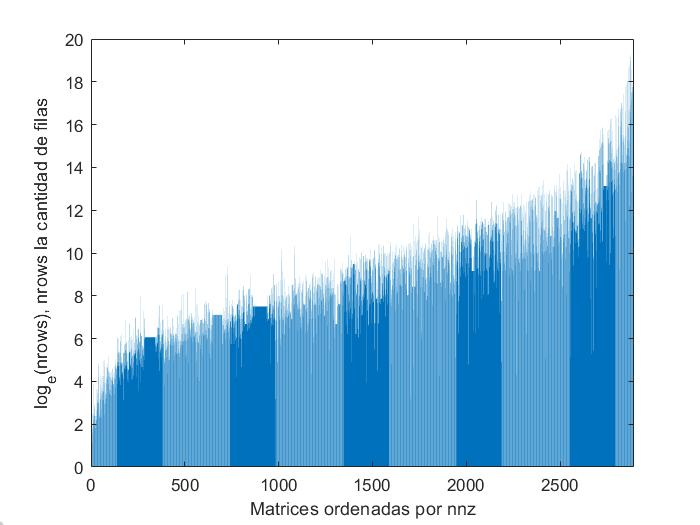
\includegraphics[width=\textwidth]{imagenes/chap4/matrix-sizes.jpg}
    \caption{Cada barra del gráfico simboliza una de las 2893 matrices ordenadas según \textit{nnz}, y su altura la dimensión de la matriz expresada logarítmicamente.}
    \label{fig:matrix-sizes}
\end{figure}
A la fecha, la SSMC está conformada por 2893 matrices de problemas diversos, con múltiples propiedades y patrones. Por ejemplo, 1407 de estas matrices presentan un patrón simétrico, 1185 de éstas tienen además simetría numérica, 601 corresponden a matrices con coeficientes binarios, entre otras posibles categorizaciones\footnote{Notar que algunas de estas clases no son excluyentes entre sí, sino que una matriz puede presentar más de una de estas propiedades}.
A su vez, las matrices pueden ser ordenadas y clasificadas por cantidad de elementos no nulos (\textit{nnz}), así como cantidad de filas y columnas.

Con respecto a la dimensión de los problemas, se pueden encontrar matrices de $2\times 2$ (no tan comunes), hasta aquellas que poseen $226.196.185 \approx e^{19.24}$	filas y columnas, tal y como se puede apreciar en el gráfico de la Figura~\ref{fig:matrix-sizes}. Y en cuanto a la cantidad de elementos no nulos, el valor máximo de \textit{nnz} es $11.588.725.964$, para una matriz de $183.964.077\times183.964.077$.



\section{Reducción de diagonales en matrices}\label{sec:ae}

Como se presentó en la Sección \ref{multiple-precision} algunos autores han utilizado técnicas de reducción del ancho de banda de las matrices para mejorar el uso de formatos de banda o híbridos. 

En un principio, se puso especial foco en la reducción de la cantidad de diagonales, de forma de poder agrupar y representar las diagonales más densas sin la necesidad de utilizar índices para cada elemento no nulo, de manera similar a la planteada en~\cite{Pinar1999} para los bloques. Si una matriz concentra una proporción importante de sus elementos no nulos en posiciones pertenecientes
a unas pocas diagonales densas, se puede dividir la misma  en dos componentes donde uno corresponde a las diagonales densas y el otro al resto de los elementos no nulos.
A continuación se resumen algunos de los esfuerzos realizados en el proyecto en este sentido.


\subsection{Heurísticas para reordenamiento}

Con la idea de verificar y estudiar la posible compresión de matrices, se desarrolla un algoritmo evolutivo capaz de evaluar y encontrar, para la matriz $M$ que se le indique, de tamaño $n \times n$, un vector de permutación $p$ (de tamaño $n$) que, al aplicarlo, minimice lo más que se pueda alguna métrica establecida de antemano, como por ejemplo el ancho de banda de la matriz o la cantidad de diagonales densas. Aplicar la permutación expresada en $p$ a una matriz $M$, implica remplazar cada fila/columna $i$ por la fila/columna $p(i)$. %Que equivalentemente representado por una matriz $P$ se obtiene la matriz $M(p,p) = P\times M \times P^t$, donde las filas y columnas están ordenadas según $p$. 

Los algoritmos evolutivos, buscan soluciones a cierto tipo de problemas sometiendo a una población de individuos a acciones y circunstancias aleatorias semejantes a las que actúan en la evolución biológica (recombinaciones y mutaciones por ejemplo), así como también a una selección de acuerdo con algún criterio, en función del cual se decide cuáles son los individuos más adaptados, que sobreviven, y cuáles los menos aptos, que son descartados. En el Anexo \ref{Ane1} se describen con mayor profundidad los conceptos básicos de estos algoritmos.

En las siguientes sub-secciones se presentan variantes del algoritmo evolutivo en un esfuerzo por encontrar y evidenciar posibles características que presentan las matrices dispersas para explotar formatos basados en diagonales.
En primer lugar, se estudia la posibilidad de reducción de ancho de banda para codificar los enteros de los índices en base a su distancia a la diagonal, buscando ahorrar espacio en el almacenamiento de los mismos. Luego, la idea fue reducir la cantidad de diagonales de las matrices, de forma de poder representar las diagonales más densas sin los índices. Dado que RCM es una heurística con objetivos similares a  estos, porque la reducción del ancho de banda está relacionada muchas veces a la cantidad de diagonales, el estudio se centra en saber si, planteando estos nuevos objetivos, existen soluciones mucho mejores que las dadas por RCM. Por esta razón, se plantean las variantes del algoritmo evolutivo.


\subsubsection{Reducción del ancho de banda}\label{sec:band-reduction-ag}

En este primer caso, con el algoritmo evolutivo se busca evaluar cuán lejos está la permutación generada por RCM de un posible reordenamiento óptimo. En otras palabras, el algoritmo se encargará de obtener, basado en la evaluación del ancho de banda de la matriz en cada iteración, una permutación de filas y columnas capaz de competir con RCM.

%Cuando se habla de un formato diagonal, se hace referencia por ejemplo, al formato DIA (abordado en la Sección \ref{dia-format}), comúnmente utilizado para matrices con anchos de banda reducidos. Parámetro que RCM intenta minimizar, de igual manera el algoritmo evolutivo en esta primer prueba.

El algoritmo diseñado trabaja sobre matrices de tamaño $n \times n$. La familia de individuos o cromosomas serán vectores de permutación de tamaño $n$. La función a minimizar (\textit{fitness}) será el ancho de banda $\beta$ de la matriz. 
Es bien sabido que una componente importante del algoritmo o estrategia evolutiva son los operadores a los cuales se somete a la población de individuos, dado que son la herramienta que permite al algoritmo alcanzar cierta meta u óptimo. 
Para este problema, dado que los genotipos son vectores de permutación, en caso de incluir operadores de cruzamiento (o recombinación) es necesario utilizar estrategias especializadas en este tipo de codificación, quedando excluidos los operadores sencillos como el de un punto de la codificación binaria. Por esta razón, y contemplando el alto costo computacional que implican estos operadores (pruebas preliminares con el operador \textit{Order Crossover}~\cite{AJ2015}) para cruzar estos individuos que presentan restricciones como por ejemplo que no se repitan valores, se decidió no explorar a fondo este camino.
 De forma de intentar reforzar la carencia del operador de cruzamiento, se implementan dos operadores de mutación: \texttt{fliplr} y \texttt{swap}. El primero consiste en invertir el orden de los elementos que componen un individuo, y se aplica a la mitad de los individuos de cada generación, seleccionados aleatoriamente. El segundo operador de mutación, que se aplica con una cierta probabilidad (\textit{Mutation rate}), consiste en realizar un intercambio (\texttt{swap}) entre dos elementos del individuo.

Para la evaluación del algoritmo evolutivo, en las primeras etapas se trabajó con matrices de dimensiones acotadas (y quizás poco representativas). Un ejemplo de estas matrices es \texttt{bfwb62}, correspondiente a un problema  de electromagnetismo, de tamaño $62 \times 62$ y 342 elementos no nulos.
\begin{figure}
\centering
\begin{subfigure}[t]{.3\textwidth}
  \centering
  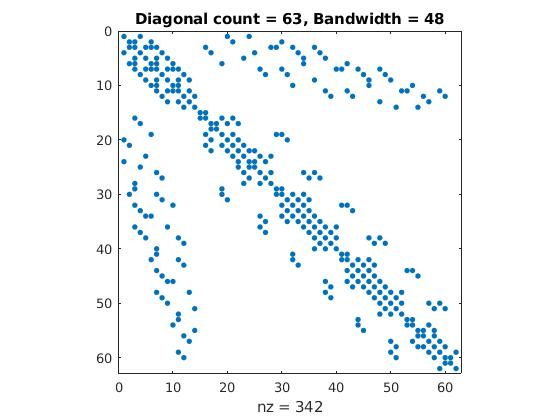
\includegraphics[width=\linewidth]{imagenes/chap4/bfwb62_spy.jpg}
  \caption{bfwb62 original.}
  \label{fig:bfwb62_spy}
\end{subfigure}%
\begin{subfigure}[t]{.3\textwidth}
  \centering
  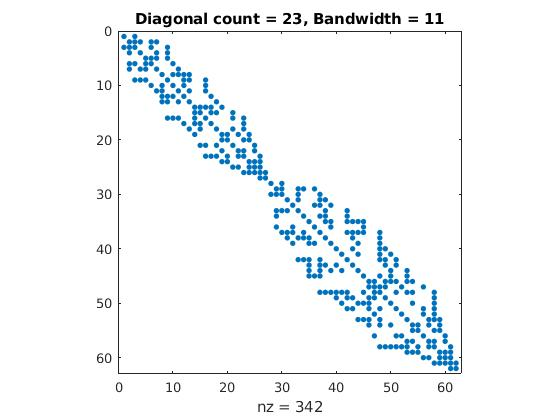
\includegraphics[width=\linewidth]{imagenes/chap4/bfwb62_rcm_spy.jpg}
  \caption{bfwb62 con RCM.}
  \label{fig:bfwb62_rcm_spy}
\end{subfigure}
\begin{subfigure}[t]{.3\textwidth}
  \centering
  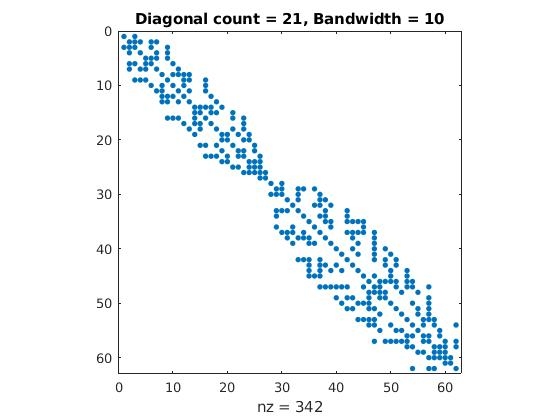
\includegraphics[width=\linewidth]{imagenes/chap4/bfwb62_ga_band_spy.jpg}
  \caption{bfwb62 con el algoritmo evolutivo.}
  \label{fig:bfwb62_ga_spy}
\end{subfigure}
\caption{Tres estados de la matriz \texttt{bfwb62} con diferentes reordenamientos.}
\label{fig:bfwb62_band}
\end{figure}
En la Figura~\ref{fig:bfwb62_band} se muestran tres instancias de la matriz con reordenamientos distintos. Pese a que las imágenes no muestran una diferencia significativa, principalmente entre RCM y la estrategia evolutiva, aplicando la permutación obtenida con el algoritmo evolutivo, se logra reducir en un elemento el ancho de banda con respecto al reordenamiento generado por RCM. 

\subsubsection*{Evaluación experimental}

El resto de las pruebas se realizaron sobre un subconjunto de matrices de problemas variados y con patrones distintos, buscando cierta heterogeneidad en las pruebas. En general, la dimensión de estas matrices es solo ligeramente mayor que la de la prueba anterior, debido a la creciente cantidad de cómputo necesaria que va a la par con la dimensión de los problemas.

Para las pruebas, el arreglo de los parámetros con los que se instanció el algoritmo evolutivo son los siguientes :
\begin{itemize}
    \item Población inicial: 240 individuos
    divididos en tres grupos, una porción de individuos o permutaciones correspondiente a la identidad, es decir, un vector que contiene de forma ordenada los valores de 1 a $n$, siendo $n$ la dimensión de la matriz, otra porción de individuos con la permutación obtenida de aplicar RCM, y el resto, la porción más grande, de permutaciones aleatorias.
    \item \textit{Generations} o cantidad máxima de generaciones: 2500,
    \item \textit{Mutation rate} o probabilidad de mutación: $0,2$,
    \item \textit{Operadores:} los dos operadores de mutación antes mencionados.
\end{itemize}

\begin{table}[h]
\resizebox{\textwidth}{!}{
\begin{tabular}{|l|r|r|r|r|r|r|r|r|r|r|r|} 
\hline
\multirow{2}{*}{\textbf{ Matriz}} & \multicolumn{1}{l|}{\multirow{2}{*}{\textbf{ Dim($n$)}}} & \multicolumn{1}{l|}{\multirow{2}{*}{\textbf{ \nnz}}} & \multicolumn{2}{c|}{\textbf{Original}}            & \multicolumn{2}{c|}{\textbf{RCM}}                 & \multicolumn{2}{c|}{\textbf{AE}}                  & \multicolumn{3}{c|}{\textbf{\bw reduction (\%)}}                                           \\ 
\cline{4-12}
                                  & \multicolumn{1}{l|}{}                                   & \multicolumn{1}{l|}{}                               & \multicolumn{1}{l|}{\dc} & \multicolumn{1}{l|}{\bw} & \multicolumn{1}{l|}{\dc} & \multicolumn{1}{l|}{\bw} & \multicolumn{1}{l|}{\dc} & \multicolumn{1}{l|}{\bw} & \multicolumn{1}{l|}{RCM - Orig.} & \multicolumn{1}{l|}{AE - Orig.} & \multicolumn{1}{l|}{AE - RCM}  \\ 
\hline \hline
'662\_bus'                    & 662                                                     & 2474                                                & 463                     & 335                     & 237                     & 118                     & 237                     & 118                     & 64.78\%                             & 64.78\%                            & 0.00\%                         \\ 
\hline
'S10PI\_n1'                   & 528                                                     & 1317                                                & 97                      & 509                     & 29                      & 14                      & 27                      & 13                      & 97.25\%                             & 97.45\%                            & 7.14\%                         \\ 
\hline
'Si2'                         & 769                                                     & 17801                                               & 1013                    & 552                     & 649                     & 324                     & 649                     & 324                     & 41.30\%                             & 41.30\%                            & 0.00\%                         \\ 
\hline
'Spectro\_10NN'               & 531                                                     & 7422                                                & 994                     & 518                     & 192                     & 96                      & 190                     & 95                      & 81.47\%                             & 81.66\%                            & 1.04\%                         \\ 
\hline
'Trefethen\_700'              & 700                                                     & 12654                                               & 21                      & 512                     & 655                     & 327                     & 655                     & 327                     & 36.13\%                             & 36.13\%                            & 0.00\%                         \\ 
\hline
'bfwb782'                     & 782                                                     & 5982                                                & 593                     & 593                     & 71                      & 35                      & 71                      & 35                      & 94.10\%                             & 94.10\%                            & 0.00\%                         \\ 
\hline
'dendrimer'                   & 730                                                     & 63024                                               & 1355                    & 708                     & 853                     & 426                     & 835                     & 417                     & 39.83\%                             & 41.10\%                            & 2.11\%                         \\ 
\hline
'dwt\_503'                    & 503                                                     & 6027                                                & 477                     & 452                     & 129                     & 64                      & 129                     & 64                      & 85.84\%                             & 85.84\%                            & 0.00\%                         \\ 
\hline
'goddardRocket'     & 831                                                     & 8498                                                & 723                     & 777                     & 575                     & 287                     & 573                     & 286                     & 63.06\%                             & 63.19\%                            & 0.35\%                         \\ 
\hline
'lowThrust\_1'                & 584                                                     & 6133                                                & 509                     & 487                     & 607                     & 303                     & 595                     & 297                     & 37.78\%                             & 39.01\%                            & 1.98\%                         \\ 
\hline
'lshp\_577'                   & 577                                                     & 3889                                                & 325                     & 563                     & 53                      & 26                      & 53                      & 26                      & 95.38\%                             & 95.38\%                            & 0.00\%                         \\ 
\hline
'lshp\_778'                   & 778                                                     & 5272                                                & 411                     & 762                     & 61                      & 30                      & 61                      & 30                      & 96.06\%                             & 96.06\%                            & 0.00\%                         \\ 
\hline
'nos6'                        & 675                                                     & 3255                                                & 7                       & 30                      & 33                      & 16                      & 33                      & 16                      & 46.67\%                             & 46.67\%                            & 0.00\%                         \\ 
\hline
'orsirr\_2'                   & 886                                                     & 5970                                                & 437                     & 554                     & 245                     & 122                     & 245                     & 122                     & 77.98\%                             & 77.98\%                            & 0.00\%                         \\ 
\hline
'steam2'                      & 600                                                     & 5660                                                & 123                     & 330                     & 152                     & 76                      & 152                     & 76                      & 76.97\%                             & 76.97\%                            & 0.00\%                         \\ 
\hline
'young4c'                     & 841                                                     & 4089                                                & 5                       & 29                      & 59                      & 29                      & 59                      & 29                      & 0.00\%                              & 0.00\%                             & 0.00\%                         \\
\hline
\end{tabular}
}
\caption{Resultados del algoritmo evolutivo intentando minimizar el \textit{bandwidth} sobre el subconjunto de matrices.}
\label{tab:band-reduction-ag-results}
\end{table}

Los resultados de la evaluación se presentan en la Tabla~\ref{tab:band-reduction-ag-results}, dónde cada fila corresponde a los resultados para cada matriz, medidos o cuantificados con los parámetros: \textit{bandwidth} (\bw) y \textit{diagonal count} (\dc). Para el análisis se pondrá foco, principalmente, en las columnas porcentuales. La columna RCM-Orig. corresponde al porcentaje de reducción de ancho de banda luego de aplicar el reordenamiento generado por RCM, comparado con la matriz original. De manera similar se presenta en la columna AE-Orig., dónde se muestran los porcentajes de reducción obtenidos por el algoritmo evolutivo con respecto al reordenamiento original. Y una columna interesante es la última, AE-RCM, que muestra el porcentaje de reducción del algoritmo evolutivo comparado con el ordenamiento de RCM. De esta tabla se puede observar que, en general, los valores de ancho de banda obtenidos con el algoritmo evolutivo no se alejaron mucho de los obtenidos mediante reordenamientos generados por la heurística RCM. Son pocos los casos en que el algoritmo logró una permutación con mejor ancho de banda que RCM y, en particular, la mejora ronda en el 1\%. Siendo, posiblemente, un indicador de que los reordenamientos obtenidos con RCM son más que aceptables, dado su razonable costo computacional y midiendo la eficacia de éste según el ancho de banda resultante. 



\subsubsection{Reducción de la cantidad de diagonales}\label{sec:diag-reduction-ag}

En esta segunda prueba para el algoritmo evolutivo, lo que se busca, es obtener permutaciones que logren reducir significativamente la cantidad de diagonales independientemente de si el ancho de banda (bandwidth) se ve optimizado o no.

Naturalmente, para este nuevo enfoque es necesaria la modificación de la función \textit{fitness}, que para este caso se corresponderá con la cantidad de diagonales luego de permutar la matriz. El resto de los aspectos del algoritmo se mantienen incambiados.

\subsubsection*{Evaluación experimental}

% Para la evaluación del algoritmo evolutivo, en las primeras etapas se trabajó con matrices de dimensiones acotadas (y quizás poco representativas). Un ejemplo de estas matrices: \texttt{bfwb62}, correspondiente a un problema  de electromagnetismo, de tamaño $62 \times 62$ y 342 elementos no nulos.
Siguiendo la metodología de evaluación utilizada en la Sección~\ref{sec:band-reduction-ag} se hizo una prueba de concepto con la matriz \texttt{bfwb62}. En la Figura~\ref{fig:bfwb62-diag}, se puede observar una mejora significativa con respecto a su ordenamiento original y el de RCM. Comparado con RCM, se logra reducir en aproximadamente 21\% la cantidad de diagonales. Incluso sin que ese sea el objetivo, se produce también una reducción en el ancho de banda, logrando una reducción de 18\% con respecto a RCM, mejor resultado que el obtenido por el algoritmo en la Sección~\ref{sec:band-reduction-ag}.

% \begin{figure}[]
%   \centering
%   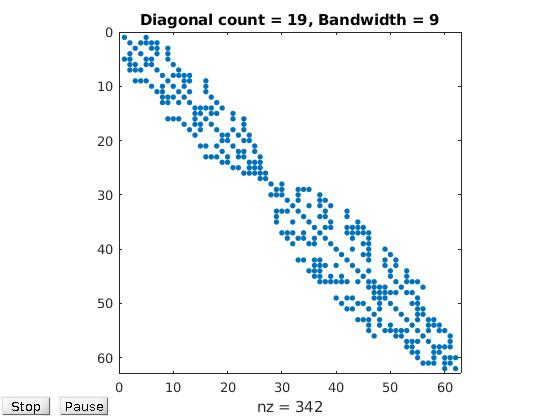
\includegraphics[width=.3\textwidth]{imagenes/chap4/bfwb62_ga_spy.jpg}
%   \caption{\texttt{bfwb62} con el algoritmo evolutivo.}
%   \label{fig:bfwb62_diag_ga_spy}
% \end{figure}

\begin{figure}
\centering
\begin{subfigure}[t]{.3\textwidth}
  \centering
  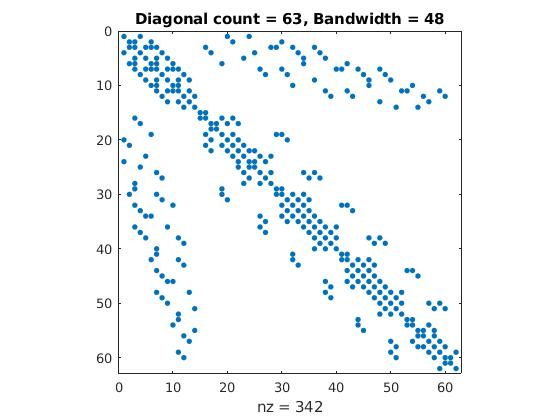
\includegraphics[width=\linewidth]{imagenes/chap4/bfwb62_spy.jpg}
  \caption{bfwb62 original.}
  \label{fig:bfwb62_spy-diag}
\end{subfigure}%
\begin{subfigure}[t]{.3\textwidth}
  \centering
  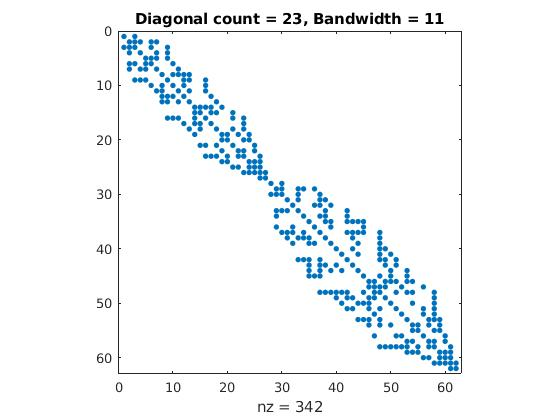
\includegraphics[width=\linewidth]{imagenes/chap4/bfwb62_rcm_spy.jpg}
  \caption{bfwb62 con RCM.}
  \label{fig:bfwb62_rcm_spy-diag}
\end{subfigure}
\begin{subfigure}[t]{.3\textwidth}
  \centering
  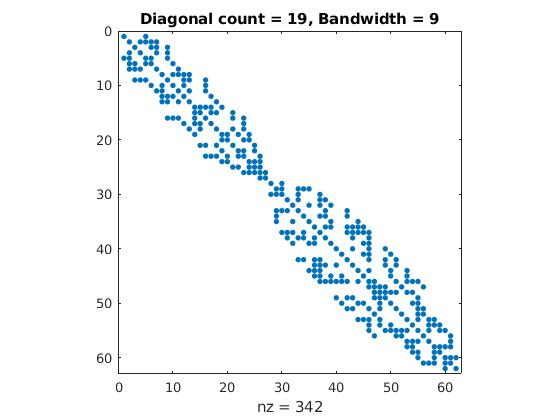
\includegraphics[width=\linewidth]{imagenes/chap4/bfwb62_ga_spy_.jpg}
  \caption{bfwb62 con el algoritmo evolutivo.}
  \label{fig:bfwb62_ga_spy-diag}
\end{subfigure}
\caption{Tres estados de la matriz \texttt{bfwb62} con diferentes reordenamientos.}
\label{fig:bfwb62-diag}
\end{figure}

% De la Figura~\ref{fig:bfwb62} se muestran tres instancias de la matriz con reordenamientos distintos. La idea es poder comparar y discutir la validez del reordenamiento obtenido con el algoritmo evolutivo. De las figuras se desprende que aplicando la permutación obtenida con el algoritmo evolutivo, se logra reducir en aproximadamente $21\%$ la cantidad de diagonales, con respecto al reordenamiento generado por RCM. 


En la etapa de evaluación de esta segunda versión de la estrategia evolutiva, se utilizó el mismo conjunto de  matrices, con la idea de obtener resultados comparativos entre los dos enfoques. Los parámetros del algoritmo, a excepción de la función de \textit{fitness} (en este caso cuenta la cantidad de diagonales), se mantienen.

Los resultados de las pruebas se pueden observar en la Tabla~\ref{tab:diag-reduction-ag-results}, análoga a la presentada en el apartado de evaluación de la Sección~\ref{sec:band-reduction-ag}.


\begin{table}[h]
\centering
\resizebox{\textwidth}{!}{
\begin{tabular}{|l|r|r|r|r|r|r|r|r|r|r|r|} 
\hline
\multirow{2}{*}{\textbf{ Matriz}} & \multicolumn{1}{l|}{\multirow{2}{*}{\textbf{ Dim($n$)}}} & \multicolumn{1}{l|}{\multirow{2}{*}{\textbf{ \nnz}}} & \multicolumn{2}{c|}{\textbf{Original}}            & \multicolumn{2}{c|}{\textbf{RCM}}                 & \multicolumn{2}{c|}{\textbf{AE}}                  & \multicolumn{3}{c|}{\textbf{\dc reduction (\%)}}                                                           \\ 
\cline{4-12}
                                  & \multicolumn{1}{l|}{}                                   & \multicolumn{1}{l|}{}                               & \multicolumn{1}{l|}{\dc} & \multicolumn{1}{l|}{\bw} & \multicolumn{1}{l|}{\dc} & \multicolumn{1}{l|}{\bw} & \multicolumn{1}{l|}{\dc} & \multicolumn{1}{l|}{\bw} & \multicolumn{1}{l|}{RCM - Orig.} & \multicolumn{1}{l|}{AE - Orig.} & \multicolumn{1}{l|}{AE - RCM}  \\ 
\hline\hline
'662\_bus'                    & 662                                                     & 2474                                                & 463                     & 335                     & 237                     & 118                     & 205                     & 118                     & 48.81\%                             & 55.72\%                            & 13.50\%                        \\ 
\hline
'S10PI\_n1'                   & 528                                                     & 1317                                                & 97                      & 509                     & 29                      & 14                      & 27                      & 13                      & 70.10\%                             & 72.16\%                            & 6.90\%                         \\ 
\hline
'Si2'                         & 769                                                     & 17801                                               & 1013                    & 552                     & 649                     & 324                     & 649                     & 324                     & 35.93\%                             & 35.93\%                            & 0.00\%                         \\ 
\hline
'Spectro\_10NN'               & 531                                                     & 7422                                                & 994                     & 518                     & 192                     & 96                      & 190                     & 95                      & 80.68\%                             & 80.89\%                            & 1.04\%                         \\ 
\hline
'Trefethen\_700'              & 700                                                     & 12654                                               & 21                      & 512                     & 655                     & 327                     & 21                      & 512                     & -3019.05\%                          & 0.00\%                             & 96.79\%                        \\ 
\hline
'bfwb782'                     & 782                                                     & 5982                                                & 593                     & 593                     & 71                      & 35                      & 71                      & 35                      & 88.03\%                             & 88.03\%                            & 0.00\%                         \\ 
\hline
'dendrimer'                   & 730                                                     & 63024                                               & 1355                    & 708                     & 853                     & 426                     & 773                     & 386                     & 37.05\%                             & 42.95\%                            & 9.38\%                         \\ 
\hline
'dwt\_503'                    & 503                                                     & 6027                                                & 477                     & 452                     & 129                     & 64                      & 129                     & 64                      & 72.96\%                             & 72.96\%                            & 0.00\%                         \\ 
\hline
'goddardRocket'     & 831                                                     & 8498                                                & 723                     & 777                     & 575                     & 287                     & 465                     & 324                     & 20.47\%                             & 35.68\%                            & 19.13\%                        \\ 
\hline
'lowThrust\_1'                & 584                                                     & 6133                                                & 509                     & 487                     & 607                     & 303                     & 427                     & 468                     & -19.25\%                            & 16.11\%                            & 29.65\%                        \\ 
\hline
'lshp\_577'                   & 577                                                     & 3889                                                & 325                     & 563                     & 53                      & 26                      & 53                      & 26                      & 83.69\%                             & 83.69\%                            & 0.00\%                         \\ 
\hline
'lshp\_778'                   & 778                                                     & 5272                                                & 411                     & 762                     & 61                      & 30                      & 61                      & 30                      & 85.16\%                             & 85.16\%                            & 0.00\%                         \\ 
\hline
'nos6'                        & 675                                                     & 3255                                                & 7                       & 30                      & 33                      & 16                      & 7                       & 30                      & -371.43\%                           & 0.00\%                             & 78.79\%                        \\ 
\hline
'orsirr\_2'                   & 886                                                     & 5970                                                & 437                     & 554                     & 245                     & 122                     & 245                     & 122                     & 43.94\%                             & 43.94\%                            & 0.00\%                         \\ 
\hline
'steam2'                      & 600                                                     & 5660                                                & 123                     & 330                     & 152                     & 76                      & 123                     & 330                     & -23.58\%                            & 0.00\%                             & 19.08\%                        \\ 
\hline
'young4c'                     & 841                                                     & 4089                                                & 5                       & 29                      & 59                      & 29                      & 5                       & 29                      & -1080.00\%                          & 0.00\%                             & 91.53\%                        \\
\hline
\end{tabular}
}
\caption{Resultados del algoritmo evolutivo intentando minimizar la cantidad de diagonales sobre sobre el subconjunto de matrices.}
\label{tab:diag-reduction-ag-results}
\end{table}



Dado que el conjunto de matrices fue elegido de modo que las mismas presenten características heterogéneas, los resultados se pueden dividir en tres grupos.
El primero de ellos, son aquellas matrices que originalmente presentan un mejor ordenamiento que el que puede generar RCM (en algunos casos tanto para cantidad de diagonales como ancho de banda). En estos casos posiblemente el ordenamiento original sea el óptimo, por lo que el algoritmo evolutivo tiende a quedarse con dicho ordenamiento original. Por ejemplo, observar las filas de la Tabla~\ref{tab:diag-reduction-ag-results} correspondientes a las matrices \texttt{Trefethen\_700} y \texttt{nos6}. 
Como segundo caso, están aquellas matrices para las cuales RCM obtiene una muy buena permutación, por ejemplo, \texttt{lshp\_577}, \texttt{lshp\_778} y \texttt{dwt503}. El efecto del algoritmo evolutivo para estos casos, es similar producido en el experimento anterior no logrando mejoras sustanciales con respecto a la solución obtenida con RCM. Observar los resultados de 0\% en la columna AE-RCM.
Y el tercer caso, el que presenta mayor interés, son aquellas que permiten evidenciar cuán lejos está RCM de un posible óptimo. Entonces, para analizar más en detalle los resultados, se centran los esfuerzos de la discusión sobre el tercer conjunto. 

De las pruebas realizadas, se puede observar que para 4 de 6 matrices para las cuales el algoritmo presenta un mejor reordenamiento que el de RCM y el original, el algoritmo evolutivo obtiene soluciones que lo sobrepasan a RCM por aproximadamente 10\%. Hay incluso, un caso donde se logra una mejora de un 29\% con respecto a RCM, y es para la matriz \texttt{lowThrust1}, donde RCM obtuvo un mal rendimiento medido en cantidad de diagonales.

En general, cuando RCM obtiene una permutación que no favorece en la cantidad de  diagonales, es decir, aumenta significativamente este valor, el resultado obtenido por el algoritmo tiende a ser similar al ordenamiento original. % (Es mas del primer caso creo...)

% matrices admiten un reordenamiento de alrededor del 10\% mejor que el generado por RCM, medido en cantidad de diagonales.


%conjunto utilizado en numerosas investigaciones para evaluar nuevas propuestas a modo de benchmark, principalmente para nuevos formatos dispersos que buscan mejorar la o SpMV~\cite{Maggioni2014,Xu2010, Bell2009, GarlandAndBell2009} (casi seguro que hay mas). (Hasta ahora, las pruebas no han salido bien, no se mueve ninguna de las cantidades para estas matrices grandes).

\subsubsection{Cantidad fija de diagonales para formatos híbridos}\label{sec:diag-perc-reduction}

Habiendo estudiado la posibilidad de reordenar las matrices intentando reducir ancho de banda y cantidad de diagonales, con un enfoque en la posible aplicación de formatos de compresión de índices%utilizando \textit{delta encoding}, como formatos de banda que almacenan la matriz por sus diagonales
, a continuación se plantea un estudio del mismo conjunto de matrices, ahora con el objetivo de emplear formatos híbridos (por ejemplo HYB, entre otros). En este caso se almacena la matriz, generalmente, en dos partes, una con una estructura razonablemente regular y la otra completamente dispersa. Modificando el algoritmo evolutivo, se intenta encontrar la permutación que, aplicada a las matrices, maximice la cantidad de elementos no nulos en cierta cantidad fija de diagonales, sin intentar optimizar el resto de parámetros. Es decir, se busca lograr una permutación que genere algunas diagonales densas (posiblemente cerca de la diagonal principal), de forma de poder almacenar las mismas en una estructura regular, en lugar de minimizar el ancho de banda y cantidad de diagonales. Notar que esta estrategia tiene cierto límite. En una matriz de tamaño $n\times n$, en el mejor de los casos, si se logra disponer los elementos en las $d$ diagonales que son más próximas a la principal, igualmente puede suceder que la cantidad de elementos no nulos de la matriz sea mayor a las entradas disponibles para $d$ diagonales. Cabe destacar que, para la evaluación, no se tomó en consideración que los elementos no nulos estuviesen en dichas diagonales próximas a la principal, sino que se calcula entre todas, la cantidad de elementos que cada una posee y posteriormente se selecciona aquellas $d$ con mayor cantidad de \textit{nnz}. 

\subsubsection*{Evaluación experimental}

Para la evaluación de esta estrategia, con respecto a las anteriores sólo cambia la función \textit{fitness}. Ahora en lugar de minimizar, como se realizó para los parámetros elegidos en las Secciones~\ref{sec:band-reduction-ag}~y~\ref{sec:diag-reduction-ag}, la función calcula la máxima cantidad de elementos no nulos en una cantidad fija de diagonales $d$, expresada en la implementación como un porcentaje de $n$. 
Para estas pruebas, el porcentaje de diagonales fue un 2\% de $n$. 
% $d = round(n/100)\times 2$, valor que depende de las dimensiones de cada matriz.

\begin{table}[]
\centering
\resizebox{\textwidth}{!}{
\begin{tabular}{|l|r|r|r|r|r|r|r|r|r|r|r|r|r|r|r|} 
\hline
\multirow{2}{*}{\textbf{Matriz}} & \multicolumn{1}{l|}{\multirow{2}{*}{\begin{tabular}[c]{@{}l@{}}\textbf{Dim} \\ \textbf{($n$)}\end{tabular}}} & \multicolumn{1}{l|}{\multirow{2}{*}{\textbf{\nnz}}} & \multicolumn{1}{l|}{\multirow{2}{*}{\begin{tabular}[c]{@{}l@{}}\textbf{2\%} \\ \textbf{DIAG}\end{tabular}}} & \multicolumn{4}{c|}{\textbf{Original}}                                                                                                                                                                               & \multicolumn{4}{c|}{\textbf{RCM}}                                                                                                                                                                                     & \multicolumn{4}{c|}{\textbf{AE}}                                                                                                                                                                                       \\ 
\cline{5-16}
                                  & \multicolumn{1}{l|}{}                                   & \multicolumn{1}{l|}{}                               & \multicolumn{1}{l|}{}                                    & \multicolumn{1}{l|}{\dc} & \multicolumn{1}{l|}{\bw} & \multicolumn{1}{l|}{\begin{tabular}[c]{@{}l@{}}NNZ IN \\2\% DIAG\end{tabular}} & \multicolumn{1}{l|}{\begin{tabular}[c]{@{}l@{}}\%NNZ IN\\ 2\%~DIAG\end{tabular}} & \multicolumn{1}{l|}{\dc} & \multicolumn{1}{l|}{\bw} & \multicolumn{1}{l|}{\begin{tabular}[c]{@{}l@{}}NNZ IN\\             2\% DIAG\end{tabular}} & \multicolumn{1}{l|}{\begin{tabular}[c]{@{}l@{}}\%NNZ IN             \\2\% DIAG\end{tabular}} & \multicolumn{1}{l|}{\dc} & \multicolumn{1}{l|}{\bw} & \multicolumn{1}{l|}{\begin{tabular}[c]{@{}l@{}}NNZ IN \\            2\% DIAG\end{tabular}} & \multicolumn{1}{l|}{\begin{tabular}[c]{@{}l@{}}\%NNZ IN             \\2\% DIAG\end{tabular}}  \\ 
\hline \hline
'662\_bus'                    & 662                                                     & 2474                                                & 14                                                       & 463                     & 335                     & 951                                                                           & 38.44\%                                                                          & 237                     & 118                     & 966                                                                            & 39.05\%                                                                          & 529                     & 651                     & 1701                                                                           & 68.76\%                                                                           \\ 
\hline
'S10PI\_n1'                   & 528                                                     & 1317                                                & 10                                                       & 97                      & 509                     & 1223                                                                          & 92.86\%                                                                          & 29                      & 14                      & 1058                                                                           & 80.33\%                                                                          & 65                      & 513                     & 1256                                                                           & 95.37\%                                                                           \\ 
\hline
'Si2'                         & 769                                                     & 17801                                               & 16                                                       & 1013                    & 552                     & 7029                                                                          & 39.49\%                                                                          & 649                     & 324                     & 4256                                                                           & 23.91\%                                                                          & 1099                    & 768                     & 7200                                                                           & 40.45\%                                                                           \\ 
\hline
'Spectro\_10NN'               & 531                                                     & 7422                                                & 10                                                       & 994                     & 518                     & 208                                                                           & 2.80\%                                                                           & 192                     & 96                      & 2182                                                                           & 29.40\%                                                                          & 340                     & 530                     & 3130                                                                           & 42.17\%                                                                           \\ 
\hline
'Trefethen\_700'              & 700                                                     & 12654                                               & 14                                                       & 21                      & 512                     & 9610                                                                          & 75.94\%                                                                          & 655                     & 327                     & 2818                                                                           & 22.27\%                                                                          & 21                      & 512                     & 9610                                                                           & 75.94\%                                                                           \\ 
\hline
'bfwb62'                      & 62                                                      & 342                                                 & 2                                                        & 63                      & 48                      & 94                                                                            & 27.49\%                                                                          & 23                      & 11                      & 86                                                                             & 25.15\%                                                                          & 83                      & 60                      & 108                                                                            & 31.58\%                                                                           \\ 
\hline
'bfwb782'                     & 782                                                     & 5982                                                & 16                                                       & 593                     & 593                     & 3733                                                                          & 62.40\%                                                                          & 71                      & 35                      & 2926                                                                           & 48.91\%                                                                          & 609                     & 597                     & 3785                                                                           & 63.27\%                                                                           \\ 
\hline
'dendrimer'                   & 730                                                     & 63024                                               & 14                                                       & 1355                    & 708                     & 8000                                                                          & 12.69\%                                                                          & 853                     & 426                     & 4551                                                                           & 7.22\%                                                                           & 1425                    & 729                     & 9168                                                                           & 14.55\%                                                                           \\ 
\hline
'dwt\_503'                    & 503                                                     & 6027                                                & 10                                                       & 477                     & 452                     & 2190                                                                          & 36.34\%                                                                          & 129                     & 64                      & 1919                                                                           & 31.84\%                                                                          & 537                     & 493                     & 2813                                                                           & 46.67\%                                                                           \\ 
\hline
'goddardRocket'     & 831                                                     & 8498                                                & 16                                                       & 723                     & 777                     & 2937                                                                          & 34.56\%                                                                          & 575                     & 287                     & 1472                                                                           & 17.32\%                                                                          & 727                     & 789                     & 4291                                                                           & 50.49\%                                                                           \\ 
\hline
'lowThrust\_1'                & 584                                                     & 6133                                                & 12                                                       & 509                     & 487                     & 2377                                                                          & 38.76\%                                                                          & 607                     & 303                     & 836                                                                            & 13.63\%                                                                          & 721                     & 547                     & 2554                                                                           & 41.64\%                                                                           \\ 
\hline
'lshp\_577'                   & 577                                                     & 3889                                                & 12                                                       & 325                     & 563                     & 2487                                                                          & 63.95\%                                                                          & 53                      & 26                      & 2680                                                                           & 68.91\%                                                                          & 277                     & 571                     & 3072                                                                           & 78.99\%                                                                           \\ 
\hline
'lshp\_778'                   & 778                                                     & 5272                                                & 16                                                       & 411                     & 762                     & 3583                                                                          & 67.96\%                                                                          & 61                      & 30                      & 3920                                                                           & 74.36\%                                                                          & 355                     & 766                     & 4310                                                                           & 81.75\%                                                                           \\ 
\hline
'nos6'                        & 675                                                     & 3255                                                & 14                                                       & 7                       & 30                      & 3255                                                                          & 100.00\%                                                                         & 33                      & 16                      & 2893                                                                           & 88.88\%                                                                          & 7                       & 30                      & 3255                                                                           & 100.00\%                                                                          \\ 
\hline
'orsirr\_2'                   & 886                                                     & 5970                                                & 18                                                       & 437                     & 554                     & 5170                                                                          & 86.60\%                                                                          & 245                     & 122                     & 2491                                                                           & 41.73\%                                                                          & 437                     & 554                     & 5170                                                                           & 86.60\%                                                                           \\ 
\hline
'steam2'                      & 600                                                     & 5660                                                & 12                                                       & 123                     & 330                     & 2413                                                                          & 42.63\%                                                                          & 152                     & 76                      & 2116                                                                           & 37.39\%                                                                          & 230                     & 595                     & 2518                                                                           & 44.49\%                                                                           \\ 
\hline
'young4c'                     & 841                                                     & 4089                                                & 16                                                       & 5                       & 29                      & 4089                                                                          & 100.00\%                                                                         & 59                      & 29                      & 2295                                                                           & 56.13\%                                                                          & 5                       & 29                      & 4089                                                                           & 100.00\%                                                                          \\
\hline
\end{tabular}
}
\caption{Resultados del algoritmo evolutivo intentando maximizar la cantidad de elementos no nulos en $d$ diagonales para cada matriz del subconjunto de matrices.}
\label{tab:max-nnz-diag-ag-results}
\end{table}

% Algunas observaciones de los resultados presentados en la Tabla~\ref{tab:max-nnz-diag-ag-results} son los siguientes: en general RCM, para las pruebas realizadas, si bien existen casos donde se logran mejora, tiende a empeorar la cantidad de elementos no nulos que van a parar en una cantidad de diagonales fija $d$ con respecto a la matriz original.
La Tabla~\ref{tab:max-nnz-diag-ag-results} muestra que, luego de aplicar los ordenamientos, RCM tiende a disminuir la cantidad de elementos no nulos en las $d$ diagonales más próximas a la principal.
Por este motivo, se hace especial foco en comparar los resultados del algoritmo evolutivo con el ordenamiento original que presentan las matrices. En general, se puede apreciar que hay una aparente mejora de unos pocos puntos porcentuales por parte del algoritmo evolutivo. También se pueden observar casos en los que no se la logra maximizar la cantidad de elementos no nulos en las $d$  diagonales en absoluto, indicando posiblemente que son matrices con estructuras diagonales, como es el caso de \texttt{nos6}, que tiene un patrón bien definido. Para 5 matrices en las que el reordenamiento original supera al de RCM, el algoritmo evolutivo logra aumentar un 3\% la cantidad de elementos no nulos alrededor de la diagonal principal. Para otras 4 matrices del conjunto de prueba, la mejora fue de un 14\%. Como máximos resultados de optimización, a 2 matrices se las logra optimizar en un 30.3\% y 39.4\%.

% En general creo que esperabamos resultados mejores, ahora voy a dejar otra corrida, no se, me parecio que estaba dejando mejores resultados...

\subsection{Resumen de los resultados obtenidos}

% \resumen{Pensaba agregar esta sección para discutir y comparar los resultados de las tres estrategias aplicadas con la estrategia evolutiva}

Observando las Tablas \ref{tab:band-reduction-ag-results} y \ref{tab:diag-reduction-ag-results}, es bastante claro cómo, al utilizar la cantidad de diagonales como función \textit{fitness}, los resultados obtenidos fueron mejores que con la estrategia del \textit{bandwidth}. Cabe destacar que, % medido no sólo según la función \textit{fitness} en cada instancia del algoritmo, sino que 
en algunos casos, %de la prueba de la Sección~\ref{sec:diag-reduction-ag} se puede apreciar que 
la reducción de diagonales también implicó una reducción del ancho de banda, obteniendo mejores resultados que en el algoritmo que emplea el ancho de banda como función \textit{fitness}. Si bien ambas estrategias no son eficientes comparadas con la mayoría de las heurísticas de reordenamiento para la reducción del ancho de banda, los resultados podrían evidenciar que quizás, en lugar de enfocar los esfuerzos en reducir directamente el ancho de banda, podría ser una mejor estrategia enfocarse en reducir la cantidad de diagonales.

Con respecto a la última idea evaluada, si bien RCM en los anteriores casos resultó ser un buen comienzo para el espacio de búsqueda de un reordenamiento opitmizado, como se puede observar en la Tabla~\ref{tab:max-nnz-diag-ag-results} este no es el caso. Esto debido, probablemente, a la naturaleza del RCM no enfocado en directamente en lograr la menor cantidad de diagonales densas posibles.


\section{Categorización de matrices (Estudio del espacio de matrices)}\label{sec:matrix-cat}

Para evaluar que tan efectivas podrían ser las técnicas de compresión de matrices dispersas basadas en la reducción de precisión para almacenar los índices, a continuación se presenta una clasificación o categorización de un gran grupo de matrices de \texttt{SuiteSparse Matrix Collection}. En particular, las matrices de la colección que son simétricas, a las que se les puede aplicar técnicas de reordenamiento para reducir su ancho de banda. Se evalúa para las matrices mencionadas, utilizando técnicas distintas, cuál es la cantidad de bits mínima con la que se podría almacenar las coordenadas si se utiliza otro valor como índice de columna. Entre las estrategias que se evalúan están, reducir la precisión de los índices actuales basados en las dimensiones de la matriz, sustituir el índice por la distancia a la diagonal, y por último utilizar la diferencia con el elemento no nulo anterior o \textit{delta encoding}.

Para esta tarea se programaron rutinas (scripts y funciones) en \texttt{MATLAB}, que accediendo a través de la \texttt{API} de SSMC obtienen las matrices simétricas, y aplican las técnicas que se describen en las siguientes secciones. 


% Posteriormente, obtenidas estas matrices permutadas y a sus correspondientes originales, se procede en la obtención de datos, calculando por ejemplo anchos de banda por filas, almacenando en el proceso parámetros de interés como son: cantidad de filas representables en diferentes precisiones, distancia máxima entre elementos no nulos consecutivos, entre otros. Obtenidos los datos, se estudian para tres rangos distintos, cuantas de las filas de cada matriz pueden ser representadas si los índices se expresan como enteros en 8, 16 y 32 bits\footnote{Notar que para el caso de diferencia a la diagonal, se necesitan representaciones de enteros con signo.}. Dando como resultados los rangos $[-2^7,2^7]$, $[-2^{15},2^{15}]$ y $[-2^{31},2^{31}]$ para el caso de la diferencia a la diagonal y  los rangos $[0,2^8 - 1]$, $[0,2^{16} - 1]$ y $[0,2^{32} - 1]$ respectivamente para el caso de la diferencia con el elemento no nulo anterior.

\subsection{Comprimir los índices de cada fila sin modificarlos}\label{col-index-compression}

El primer estudio planteado consistió en evaluar la capacidad de compresión al utilizar los índices originales asociados %a cada elemento directamente si la matriz dispersa estuviese almacenada en 
al formato comprimido, ya sea por filas o columnas (incluso COO). Lo importante es que se intenta atacar la componente no comprimida de los índices. Para este caso particular, las matrices están en formato CCS, por lo que se intentarán comprimir los índices de fila, los cuales son no-negativos. El estudio evalúa la cantidad mínima de bits (8, 16 o 32) para almacenar todos los coeficientes de la matriz. Es decir, se busca el índice que requiere más bits para ser representado y, en base a esto, se cuantifican los bits necesarios para la matriz. Notar que en este caso la cantidad de bits está dada por la dimensión de la matriz, que es el máximo valor que los coeficientes pueden alcanzar. 

Como los índices a estudiar son no-negativos, y se quiere evaluar la posibilidad de utilizar representaciones con 8, 16 y 32 bits, se obtienen los siguientes rangos para poder clasificar cada matriz según sus índices máximos: $[0,2^8 - 1]$, $[0,2^{16} - 1]$ y $[0,2^{32} - 1]$.

\begin{figure}[h]
    \centering
    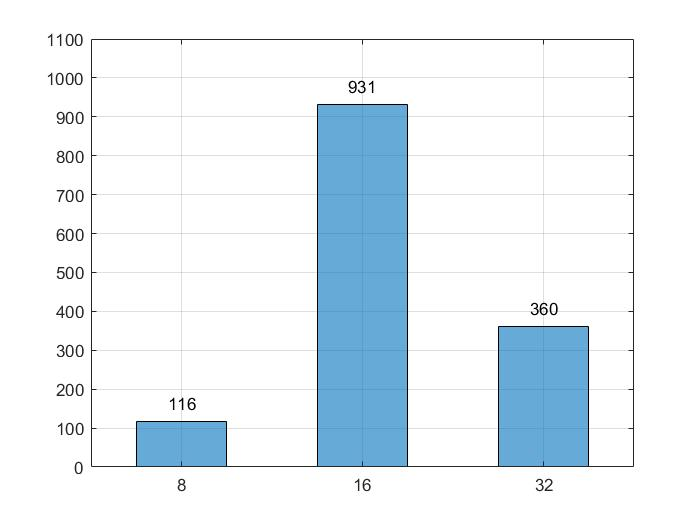
\includegraphics[width=.6\textwidth]{imagenes/chap4/hist_dim_cat.jpg}
    \caption{Histograma que muestra la cantidad de matrices cuyos índices de columna pueden ser representados en 8, 16 y 32 bits%, respectivamente, sin realizar modificaciones a la matriz, determinando los valores máximos, la dimensión de ésta
    .}
    \label{fig:hist_dim_cat}
\end{figure}

En la Figura \ref{fig:hist_dim_cat} se presenta un gráfico con la clasificación de las matrices, dependiendo de si sus índices pueden ser almacenados en cada una de las precisiones. Se puede observar que, del espacio de 1407 matrices estudiadas, quedan catalogadas con 8, 16 y 32 bits, 116, 931 y 360 matrices, respectivamente. Es decir que aproximadamente el $25\%$ de las matrices necesitan 32 bits para ser almacenadas. 

\begin{figure}[h]
    \centering
    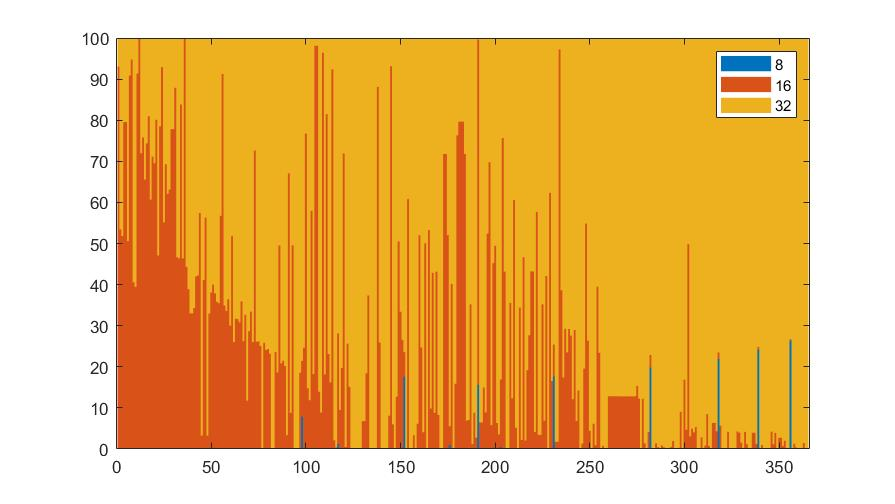
\includegraphics[width=.7\textwidth]{imagenes/chap4/index_bar_row_porc_per_cat_32.jpg}
    \caption{Cada barra del gráfico simboliza una matriz original, que necesita 32 bits para ser representada, y cada componente es el porcentaje de índices máximos por fila que pueden ser representadas con 8, 16 y 32 bits.}
    \label{fig:index_bar_row_porc_per_cat_32}
\end{figure}

En esta y en las secciones posteriores, se estudiarán con mayor foco las matrices que dependiendo de la técnica de compresión analizada, pertenecen a la categoría de 32 bits.  En este sentido, se presenta en la Figura~\ref{fig:index_bar_row_porc_per_cat_32} los resultados para dichas matrices, para observar efectivamente cuántas son las filas que necesitan los 32 bits para ser representadas, o dicho de otra forma, comparar la cantidad de filas que puedan ser representadas con 8 y 16 bits, dentro de las matrices de esta categoría. 
Las barras del gráfico están subdivididas en 3 partes, 
%Las barras del gráfico representan las matrices que pertenecen a la categoría de 32 bits, es decir, aquellas matrices que tienen alguna fila con índice máximo mayor a  $2^{16} - 1$. En particular, cada barra está subdividida en 3 partes,
indicando la proporción de filas de la matriz que pueden ser representadas con las cantidades de bits antes mencionadas. Notar como la división de los porcentajes de filas, está principalmente distribuida, en la mayoría de las matrices, entre 16 y 32 o, en otras palabras, pocas son las matrices que presentan una porción considerable de filas representables con 8 bits (si fueran una cantidad reducida de filas se podrían utilizar formatos híbridos, almacenando esas pocas filas representables con 32 en otra estructura y el resto con precisiones reducidas). Se puede apreciar, que cuanto menor es la cantidad de elementos no nulos, (izquierda del gráfico), menor es la cantidad de filas que necesitan 32 bits para ser almacenadas. A medida que crece dicha cantidad, hacia la derecha, parece aumentar progresivamente la cantidad de filas en 32 bits.



\subsection{Diferencia a la diagonal}\label{diagonal-dif}

Comenzando a evaluar posibles técnicas de compresión enfocadas sobre los índices. %Inspirado en las propuestas de Xu et al.~\cite{Xu2010},
En esta sección se realiza un estudio de la utilización de la diferencia a la diagonal como índice, en lugar del valor de columna original. Para dicho objetivo, es necesario calcular para cada fila de cada una de las matrices, la máxima distancia de un elemento no nulo a la diagonal (en valor absoluto, notar que es equivalente al ancho de banda por fila $\beta (A_i)$). Obtenidos estos valores, se determina cuantos bits son los necesarios  para su almacenamiento y se los clasifica. En este sentido, la Figura~\ref{fig:hist_diag_dist_cat} resume la cantidad de matrices que necesitan 8, 16 y 32 bits para ser almacenadas utilizando esta técnica para representar el índice. 

\begin{figure}[h]
  \centering
  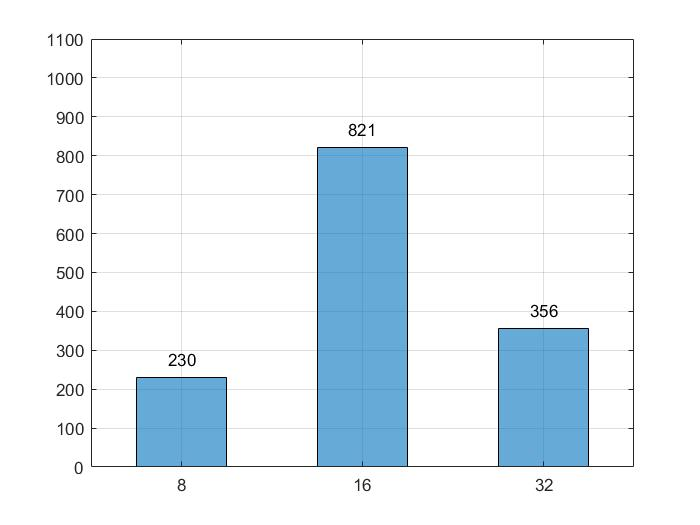
\includegraphics[width=.6\textwidth]{imagenes/chap4/hist_diag_dist_cat.jpg}
  \caption{%Histograma que muestra la clasificación de las matrices originales, según si se les puede aplicar una compresión de índice de columna basados en la distancia a la diagonal con 8, 16 y 32 bits.
  Histograma que muestra la cantidad de matrices cuyos índices de columna expresados como la distancia a la diagonal pueden ser representados en 8, 16 y 32 bits.}
  \label{fig:hist_diag_dist_cat}
\end{figure}%


Notar cómo, a diferencia de la estrategia analizada anteriormente, donde los índices sólo trabajaban con valores positivos, para esta técnica se necesitarán enteros con signo\footnote{Por ejemplo, el índice de una entrada no nula a la derecha de la diagonal tomará valores positivos, mientras que si está a la izquierda negativos.}. En particular, se busca un rango simétrico con respecto a 0, valor que simboliza la diagonal. Se obtienen para 8, 16 y 32 bits los rangos: $[-2^7,2^7]$, $[-2^{15},2^{15}]$ y $[-2^{31},2^{31}]$.



% Se me había ocurrido, modificar un cacho mas el formato, capaz que agrega overhead de descompresión después, pero tener un bit para decir de que lado esta de la diagonal y así tener un bit mas para manejar solo enteros positivos. Básicamente usar el bit de signo, por separado.

\begin{figure}[h!]
    \centering
    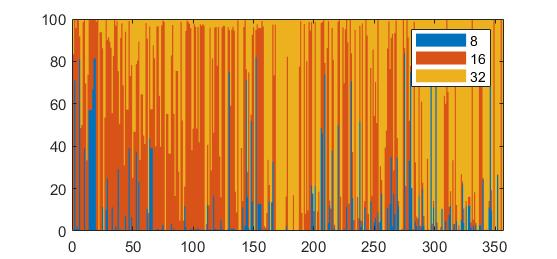
\includegraphics[width=.8\textwidth]{imagenes/chap4/bar_row_porc_per_cat_32.jpg}
    \caption{Cada barra del gráfico simboliza una matriz sin reordenar, que necesita 32 bits para ser representada, y cada componente es el porcentaje de distancias máximas por fila a la diagonal que pueden ser representadas con 8, 16 y 32 bits.}
    \label{fig:bar_row_porc_per_cat_32}
\end{figure}

 En la Figura~\ref{fig:bar_row_porc_per_cat_32}, de manera similar a la anterior sección,  se puede observar un gráfico de barras, del que se desprende que para la gran mayoría de las matrices que pertenecen a la categoría de 32 bits, a medida que crece la cantidad de elementos nulos (hacia la derecha), aumenta el porcentaje de filas en la categoría de 32 bits. También se puede observar cómo decrece el porcentaje de filas en 16 bits, notorio en la porción con menor cantidad de elementos no nulos, agrupada a la izquierda.
 
%  \resumen{Está medio pobre esto creo, no se me opcurre que otra cosa concluir}

\subsection{Diferencia a la diagonal con reordenamiento}\label{diagonal-dif-rcm}

En esta sección, se realiza un análisis del uso de técnicas de reordenamiento. En particular, y siguiendo las ideas propuesta por Xu et al.~\cite{Xu2010}, se aplica la heurística RCM a la técnica de utilizar la diferencia a la diagonal en lugar del índice de columna, presentada en la Sección~\ref{diagonal-dif}.


% \begin{figure}
% \centering
% \begin{subfigure}{.5\textwidth}
%   \centering
%   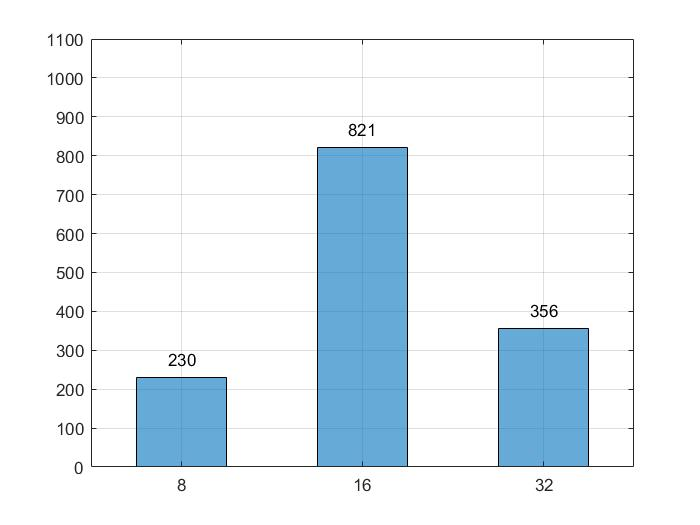
\includegraphics[width=\linewidth]{imagenes/chap4/hist_diag_dist_cat.jpg}
%   \caption{Matrices sin RCM}
%   \label{fig:hist_diag_dist_cat}
% \end{subfigure}%
% \begin{subfigure}{.5\textwidth}
%   \centering
%   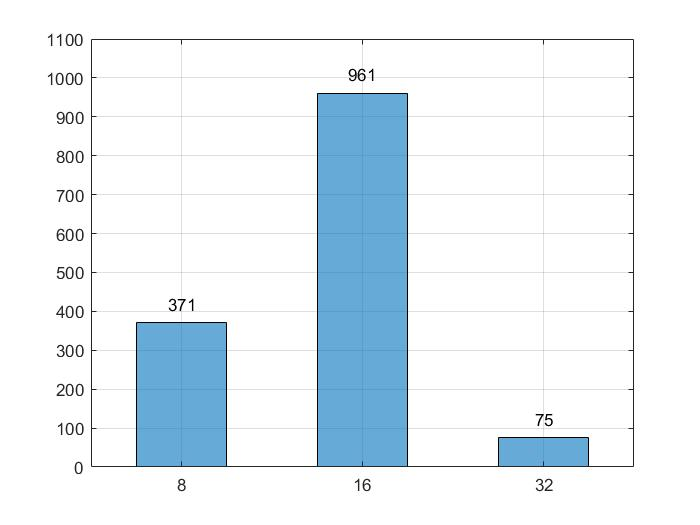
\includegraphics[width=\linewidth]{imagenes/chap4/hist_diag_dist_cat_rcm.jpg}
%   \caption{Matrices con RCM}
%   \label{fig:hist_diag_dist_cat_rcm}
% \end{subfigure}
% \caption{Histogramas donde se muestra la clasificación de las matrices según si se les puede aplicar una compresión de índice de columna basados en la distancia a la diagonal con 8, 16 y 32 bits. Matrices originales~\ref{fig:hist_diag_dist_cat} y con RCM~\ref{fig:hist_diag_dist_cat_rcm}.}
% \label{fig:hist_diag_dist}
% \end{figure}

\begin{figure}[h]
  \centering
  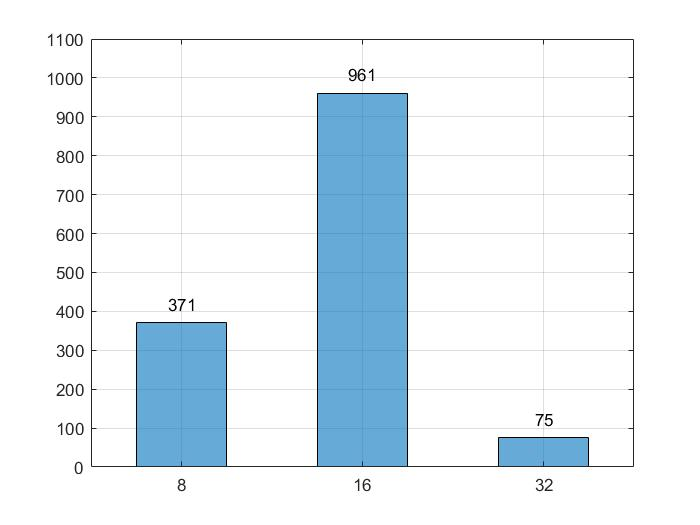
\includegraphics[width=.6\textwidth]{imagenes/chap4/hist_diag_dist_cat_rcm.jpg}
  \caption{
  Histograma que muestra la cantidad de matrices. luego de aplicar RCM, cuyos índices de columna expresados como la distancia a la diagonal pueden ser representados en 8, 16 y 32 bits.
  %Histograma donde se muestra la clasificación de las matrices luego de aplicar RCM, según si se les puede aplicar una compresión de índice de columna basados en la distancia a la diagonal con 8, 16 y 32 bits.
  }
  \label{fig:hist_diag_dist_cat_rcm}
\end{figure}%

Una comparativa de cuántas matrices son representables, utilizando la técnica de distancia a la diagonal, con 8, 16 y 32 bits, con y sin aplicación de reordenamiento, se puede observar en las Figuras \ref{fig:hist_diag_dist_cat} y \ref{fig:hist_diag_dist_cat_rcm}. De las gráficas se deduce que el uso de RCM ofrece importantes beneficios, en especial disminuyendo las matrices representables con 32 bits. Este artilugio, permite pasar de 353 a 63 matrices, del espacio representables con 32 bits, en otras palabras, 290 o el 82\% de dichas matrices se puede almacenar con precisiones menores, siempre y cuando se les aplique un reordenamiento. En el caso de 16 bits, si bien crece el número, muchas de estas son matrices que antes necesitaban 32 bits. De hecho, 154 matrices que necesitaban 16 pasan a 8 bits al aplicar RCM, como se puede observar en la  Figura~\ref{fig:confusion_diag_dist}. Este gráfico, que a los efectos de este proyecto se llamará matriz de composición, es útil para comparar los beneficios de aplicar algún tipo de reordenamiento a una técnica. Cada una de las filas representa la cantidad de matrices que originalmente pueden ser representadas utilizando el número de bits indicada por la fila, a su vez, cada una está subdividida en las categorías a las que van a parar luego de aplicar RCM. Si se la ve por columnas, cada una representa el número de matrices originales que fueron a parar a cada categoría luego de aplicado el reordenamiento obtenido con RCM. %Cuando se accede por columnas, se puede observar la cantidad de matrices en cada precisión luego de reordenar. 
En dicha figura se puede apreciar que, si bien los números del triángulo superior son muy bajos, hay valores por encima de 0 (y uno sólo en 0), indicando que algunas de éstas matrices, en su forma original, pueden ser representadas con una menor cantidad de bits que cuando se les aplica RCM. Para este caso hay 15 matrices que pasan de 8 a 16 bits, y 2 que pasan de 16 a 32. Notar que son cantidades mucho menores a aquellas que si permiten una compresión. De todos modos, evidencia que existen ciertos problemas para los que no sería conveniente aplicar esta técnica de reordenamiento.

\begin{figure}[h]
    \centering
    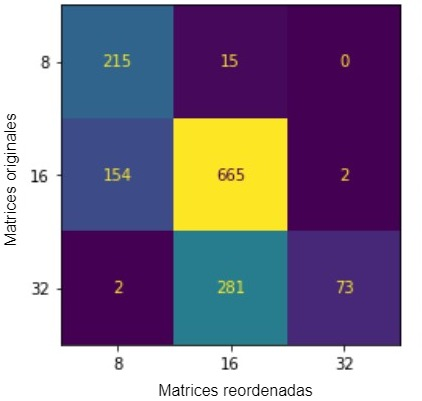
\includegraphics[width=0.4\textwidth]{imagenes/chap4/confusion_diag_dist.jpg}
    \caption{Matriz de composición, muestra en cada fila la distribución de las matrices en cada categoría luego del reordenamiento con RCM, en base a la distancia a la diagonal.}
    \label{fig:confusion_diag_dist}
\end{figure}


\begin{figure}
    \centering
    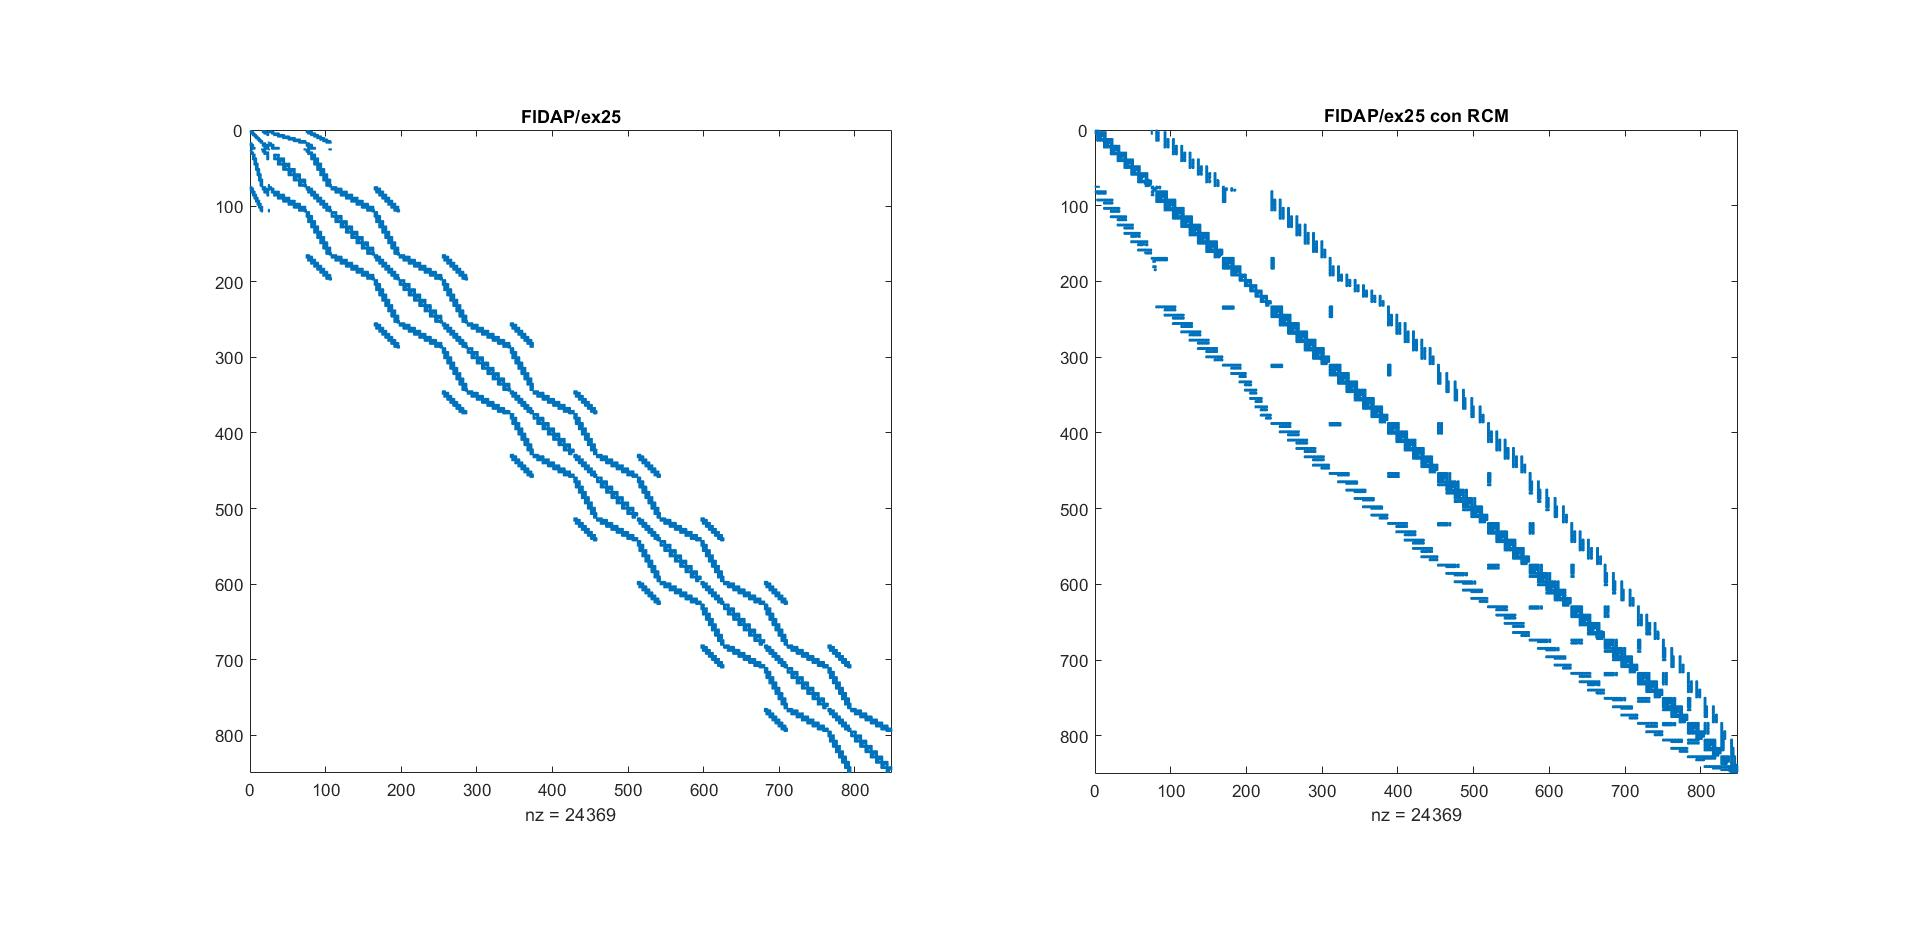
\includegraphics[width=.7\textwidth]{imagenes/chap4/spy_diag_8_to_16.jpg}
    \caption{Ejemplo de matriz que al aplicarle RCM pasa de categoría, de 8 a 16 basado en la diferencia a la diagonal.}
    \label{fig:spy_diag_8_to_16}
\end{figure}


En la Figura~\ref{fig:spy_diag_8_to_16} se presenta el ejemplo de la matriz \texttt{FIDAP/ex25} que pasa, luego de aplicar el reodenamiento generado por RCM, de la categoría de 8 a 16 bits. En particular en el ordenamiento original, las 848 filas eran representables con 8 bits, pasando a tener 475 en esta categoría y 373 en la de 16 bits. Notar la periodicidad de la matriz, estructura que se pierde por  la forma en la que reordena RCM, que pasando de vértices de grados menores a mayores, acaba por producir un leve ensanchamiento en el ancho de banda, rompiendo con la regularidad del ordenamiento original. 



\begin{figure}
    \centering
    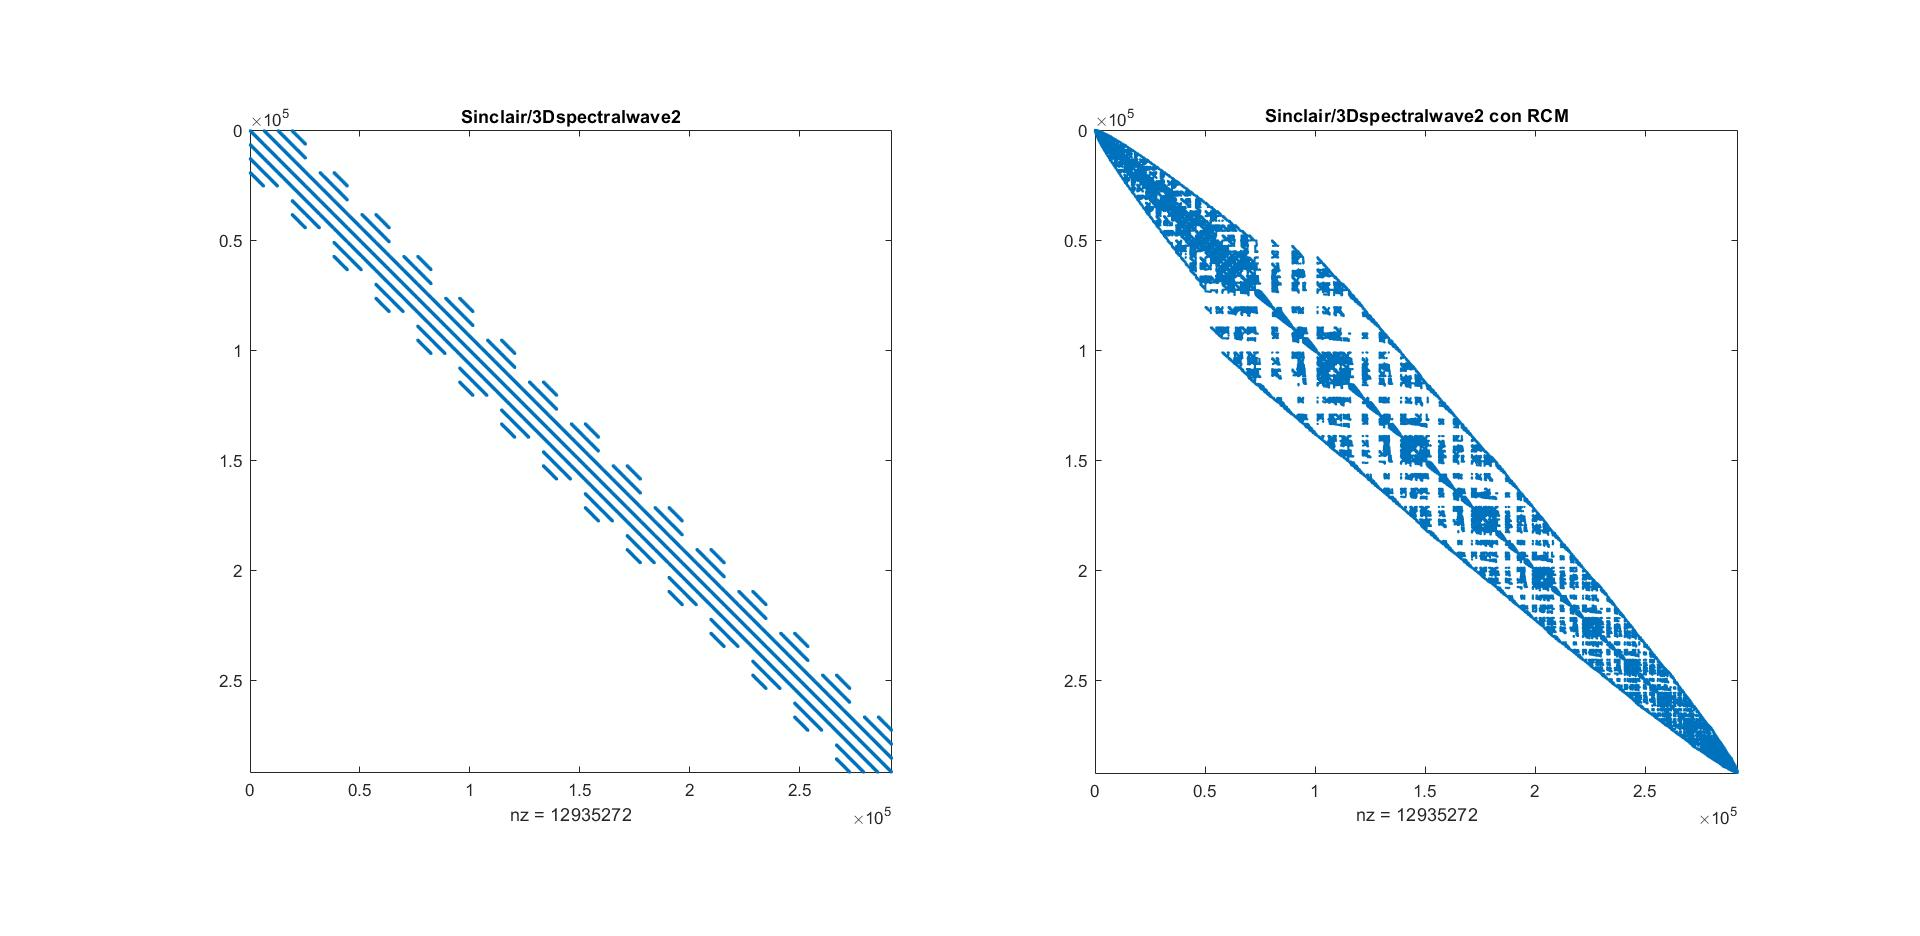
\includegraphics[width=.7\textwidth]{imagenes/chap4/spy_diag_16_to_32.jpg}
    \caption{Ejemplo de matriz que al aplicarle RCM pasa de categoría, de 16 a 32 basado en la diferencia a la diagonal.}
    \label{fig:spy_diag_16_to_32}
\end{figure}

De igual forma, en la Figura~\ref{fig:spy_diag_16_to_32} se plantea un ejemplo de matriz que pasa, en este caso, de 16 a 32 bits. \texttt{Sinclair/3Dspectralwave2} tiene un comportamiento muy similar al ejemplo anterior ante RCM.




% De esto se puede concluir que RCM, puede incluso empeorar el reordenamiento original...... SEGUIR

De esto se puede concluir que en general el uso de las heurísticas de reordenamiento, en particular RCM, permiten ahorrar en el almacenamiento. Sin embargo, es necesario estudiar caso a caso porque en algunos ejemplos de matrices estructuradas, el reordenamiento rompe con dicha estructura llegando a aumentar los requerimientos de almacenamiento, obteniendo resultados contrarios al objetivo.


\begin{figure}[h]
    \centering
    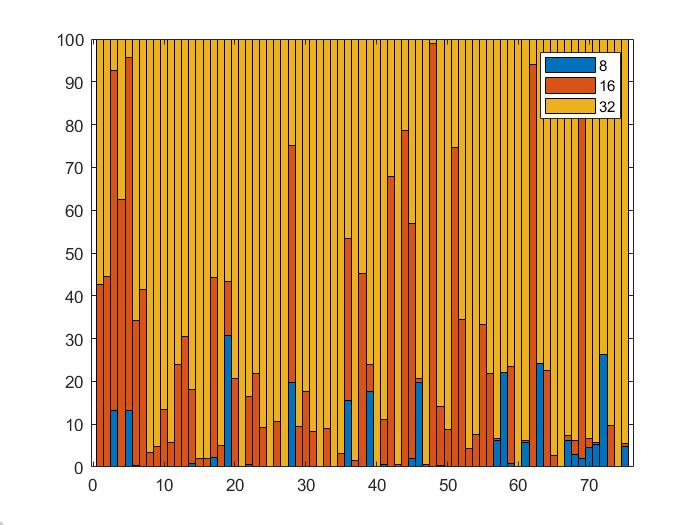
\includegraphics[width=.8\textwidth,height=.5\textwidth]{imagenes/chap4/bar_row_porc_per_cat_32_rcm.jpg}
    \caption{Cada barra del gráfico simboliza una matriz que necesita 32 bits para ser representada luego de aplicar RCM, y cada componente es el porcentaje de distancias máximas por fila a la diagonal que pueden ser representadas con 8, 16 y 32 bits.}
    \label{fig:bar_row_porc_per_cat_32_rcm}
\end{figure}

Buscando profundizar el estudio, tal y como se realizó en los casos anteriores, se toman las matrices representables con al menos 32 bits y se evalúa qué proporción de sus filas, intentando comprimirlas, permiten un cambio de precisión, es decir, una compresión. % Notar que hasta ahora, si una fila necesita 32 bits para ser indexada la matriz entera se considera de dicha categoría.
Resultados que se pueden observar en la Figura~\ref{fig:bar_row_porc_per_cat_32_rcm}, que en general indican que luego de aplicar RCM, las matrices que pertenecen a esta categoría, en su gran mayoría tienen una baja proporción de sus filas representables en precisiones menores que 32 bits. Tampoco se aprecia una correlación importante entre la cantidad de elementos no nulos y la cantidad de filas en precisiones menores.




\subsection{Delta entre índices}\label{delta}

%\resumen{deta\_max por fila}

% Además de clasificar las matrices según la cantidad de bits necesarios para almacenar en un formato donde el índice de columna se cambia por la distancia a la diagonal permitiendo 

Se estudió también, para cada matriz del conjunto definido, el delta o la distancia máxima entre elementos no nulos consecutivos para cada una de las filas y para cada matriz. % Esto, con el objetivo de observar efectivamente cuantas de las matrices dispersas con y sin la aplicación de reordenamientos, son candidatas para una compresión sobre los índices de columna, como la realizada 
Esta idea fue aplicada por Maggioni et al.~\cite{Maggioni2014}, para su formato CoAdELL, presentado de forma breve en el Capítulo~\ref{ch:estado-del-arte}, así como Kourtis et al.~\cite{Kourtis2008} en su formato CSR-DU, entre otros autores~\cite{Tang2013, Willcock2006}.

Al igual que en el estudio de los índices máximos por filas, presentado en la Sección~\ref{col-index-compression}, los valores que toman los índices utilizando este enfoque, son también positivos, notar que el elemento anterior necesariamente tendrá un índice menor, por lo que su resta será positiva.

\begin{figure}[h]
  \centering
  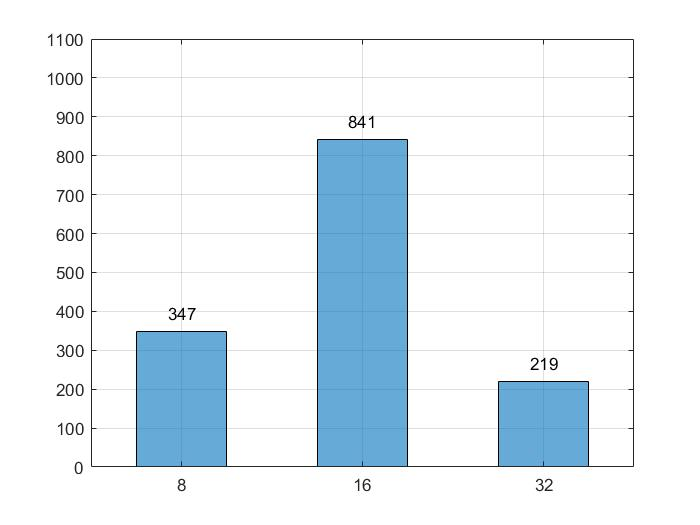
\includegraphics[width=.6\textwidth]{imagenes/chap4/hist_delta_dist_cat.jpg}
  \caption{%Histograma con la clasificación de las matrices, categorizadas según si se les puede aplicar una compresión de índice de columna basados en la distancia al elemento anterior no nulo utilizando 8, 16 y 32 bits
  Histograma que muestra la cantidad de matrices cuyos índices de columna expresados como la distancia al elemento anterior no nulo pueden ser representados en 8, 16 y 32 bits.
  }
  \label{fig:hist_delta_dist_cat}
\end{figure}%

A continuación se presentan algunos de los resultados obtenidos. En la Figura~\ref{fig:hist_delta_dist_cat} se muestra la categorización del espacio de matrices si se representa el índice como la diferencia con el anterior no nulo. Notar que, con respecto a la técnica de diferencia a la diagonal sin reordenar (Figura~\ref{fig:hist_diag_dist_cat}), aplicando esta compresión se obtienen significativamente más matrices en la categoría de 8 bits, mientras que la de 32 bits se ve reducida en un porcentaje similar.% Se mantiene el mismo patrón antes identificado, donde las matrices que pertenecen a esta categoría presentan un gran porcentaje de sus filas representables únicamente en 32 bits.



Cabe destacar que en este caso, los rangos de representación comienzan en cero (a diferencia de los rangos de la parte anterior, que utilizaban representaciones con signo),  permitiendo utilizar 1 bit más dedicado, no al signo, sino a la numeración directamente.

\begin{figure}
    \centering
    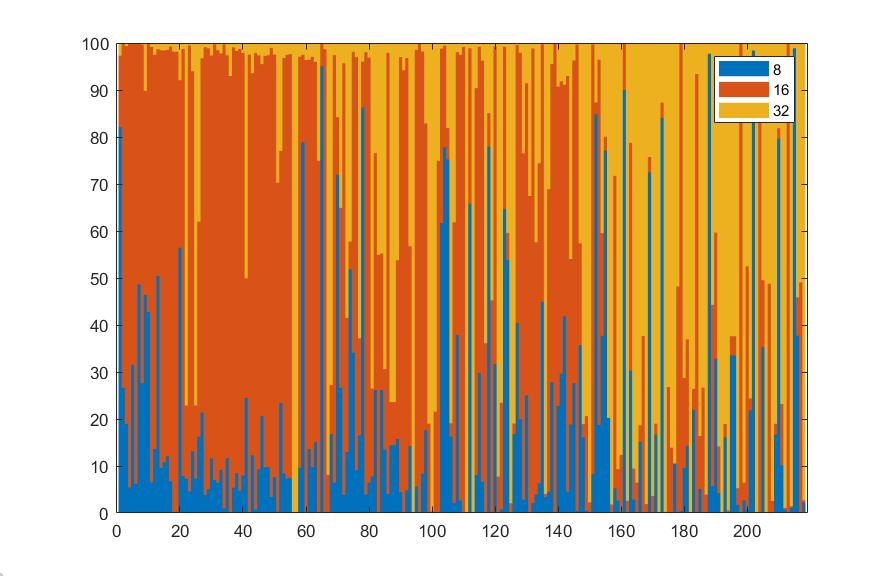
\includegraphics[width=.8\textwidth]{imagenes/chap4/delta_bar_row_porc_per_cat_32.jpg}
    \caption{Cada barra del gráfico simboliza una matriz sin reordenar, que necesita 32 bits para ser representada, y cada componente es el porcentaje de deltas máximos por fila que pueden ser representadas con 8, 16 y 32 bits.}
    \label{fig:delta_bar_row_porc_per_cat_32}
\end{figure}

Similar a lo que se realizó anteriormente, se evalúan las matrices que necesitan 32 bits para ver cuántas filas de esas matrices se pueden representar con 8 y 16 bits. Dicho estudio se resume en la Figura~\ref{fig:delta_bar_row_porc_per_cat_32}. Nuevamente, se puede observar cómo, para las matrices que poseen menores cantidades de \textit{nnz}, ubicadas sobre la izquierda del gráfico, una gran porción presenta muy pocas filas que necesitan 32 bits. A medida que aumenta la cantidad de elementos no nulos de las matrices se puede apreciar, quizás no tan regularmente, un progresivo aumento de las filas en 32 bits.


\subsection{Delta entre índices con reordenamiento}\label{delta-rcm}

\begin{figure}
  \centering
  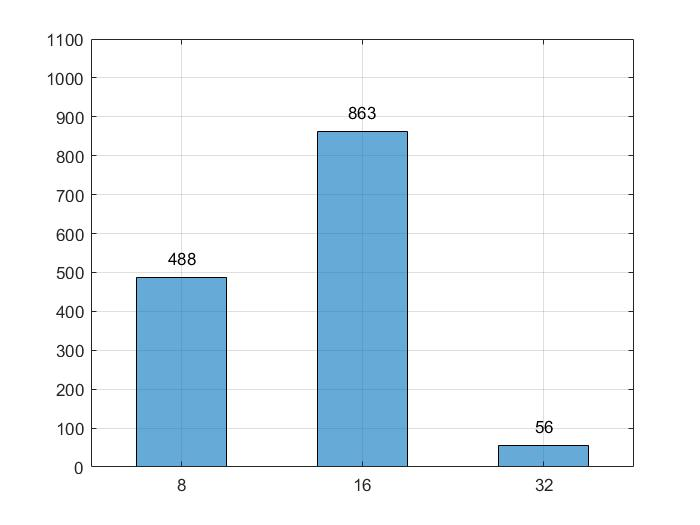
\includegraphics[width=.6\textwidth]{imagenes/chap4/hist_delta_dist_cat_rcm.jpg}
  \caption{%Histograma con la clasificación de las matrices reordenadas con RCM, categorizadas según si se les puede aplicar una compresión de índice de columna basados en la distancia al elemento anterior no nulo utilizando 8, 16 y 32 bits
   Histograma que muestra la cantidad de matrices, luego de aplicar RCM, cuyos índices de columna expresados como la distancia al elemento anterior no nulo pueden ser representados en 8, 16 y 32 bits.
  }
  \label{fig:hist_delta_dist_cat_rcm}
\end{figure}%

Considerando los importantes beneficios de usar RCM para la técnica de sustituir los índices por la diferencia a la diagonal, presentado en \ref{diagonal-dif-rcm}, en este trabajo se propone extender las ideas de Maggioni et al. aplicando RCM pero, en este caso, en conjunto con la codificación delta de forma similar a la propuesta por~\cite{Tang2013}, los resultados se resumen en la Figura~\ref{fig:hist_delta_dist_cat_rcm}.

Para esta conjunción de técnicas, se produce un efecto similar al ocurrido en la Sección~\ref{diagonal-dif-rcm}. Aplicar el reordenamiento de RCM produce resultados mejores, incluso con un impacto más positivo si se comparan los efectos sobre la técnica de la diferencia a la diagonal, obteniendo menores cantidades de matrices en la categoría de 32 bits y mayores en la de 8 bits. Con respecto a las originales con la misma técnica de la distancia al anterior, se logra reducir en aproximadamente  un $75\%$ la cantidad de matrices que se representaban originalmente con 32 bits.


\begin{figure}
    \centering
    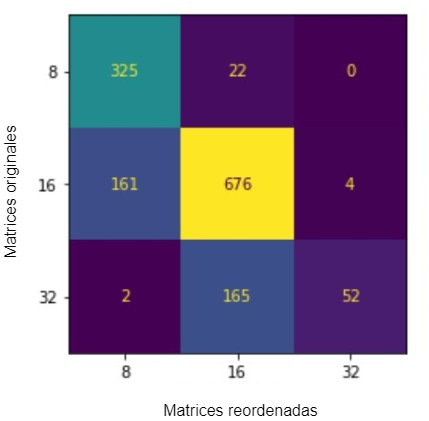
\includegraphics[width=0.4\textwidth]{imagenes/chap4/confusion_delta_dist.jpg}
    \caption{Matriz de composición, muestra en cada fila la distribución de las matrices en cada categoría luego del reordenamiento con RCM, en base a la diferencia con el elemento no nulo anterior.}
    \label{fig:confusion_delta_dist}
\end{figure}


De la misma manera, algunas matrices aumentaron la cantidad de bits necesaria para  poder ser representadas luego de aplicar el reordenamiento de RCM. Estos resultados  se pueden observar en la matriz de composición, presentada en la Figura~\ref{fig:confusion_delta_dist}. En este caso, las relaciones por encima de la diagonal corresponden a 22 matrices que pasan de 8 a 16 bits y 4 que pasan de 16 a 32. Notar que, estos son valores mayores a los obtenidos con la técnica de la diferencia a la diagonal. %Pero, estos resultados no deberían sorprender, dado que con el algoritmo evolutivo se podía apreciar un fenómeno similar, en particular para
\begin{figure}
    \centering
    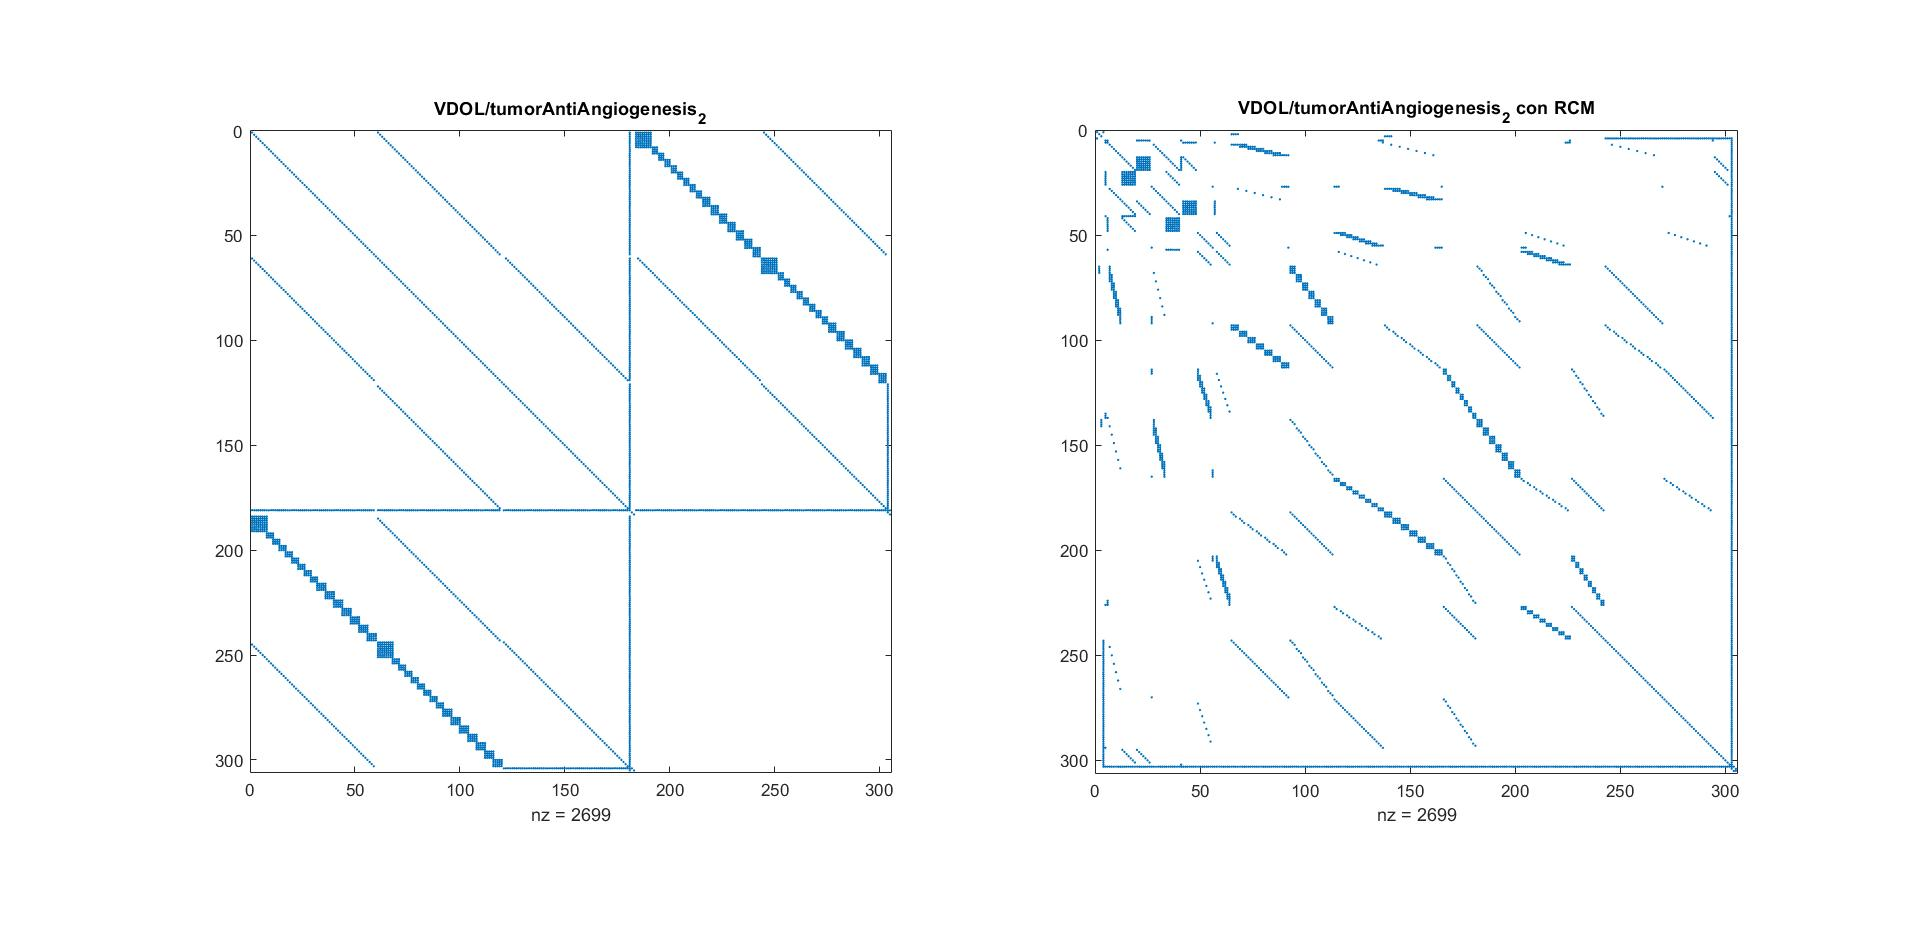
\includegraphics[width=.7\textwidth]{imagenes/chap4/spy_delta_8_to_16.jpg}
    \caption{Ejemplo de matriz que al aplicarle RCM pasa de categoría, de 8 a 16 basado en la diferencia al elemento no nulo anterior.}
    \label{fig:spy_delta_8_to_16}
\end{figure}
\begin{figure}
    \centering
    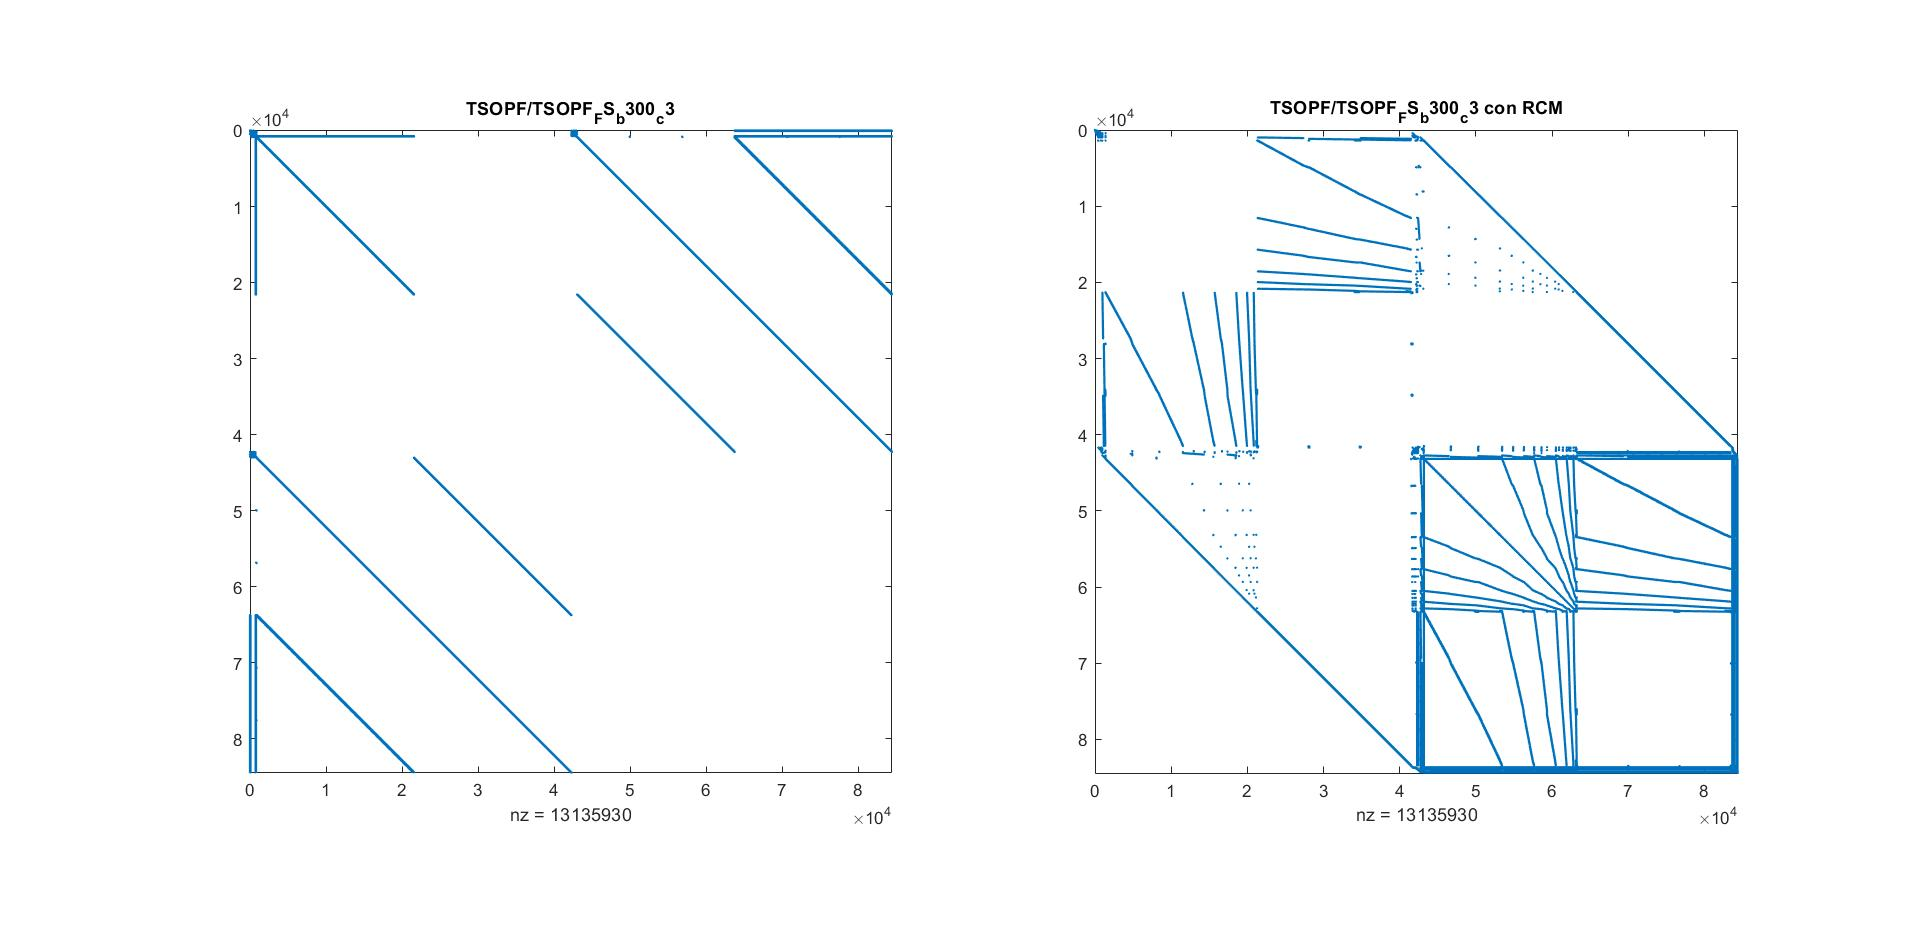
\includegraphics[width=.7\textwidth]{imagenes/chap4/spy_delta_16_to_32.jpg}
    \caption{Ejemplo de matriz que al aplicarle RCM pasa de categoría, de 16 a 32 basado en la diferencia al elemento no nulo anterior.}
    \label{fig:spy_delta_16_to_32}
\end{figure}
En las Figuras~\ref{fig:spy_delta_8_to_16} y \ref{fig:spy_delta_16_to_32} se presentan dos ejemplos de matrices que padecieron esta situación. La Figura~\ref{fig:spy_delta_8_to_16} corresponde a la matriz \texttt{VDOL/tumorAntiAngiogenesis\_2} (la imagen a la izquierda corresponde a la matriz original y la derecha a la misma luego de aplicar RCM), pasando de una distancia máxima de 180 (representable con 8 bits 0-255) entre elementos contiguos en una misma fila, a 283 (con 8 bits no es suficiente). Si bien puede dar la impresión de que, en el desorden, las distancias entre elementos no nulos se acortaron, con un estudio minucioso se  puede observar que no es así, constatando la existencia de filas que tienen distancias mayores a la original.

De igual forma, la Figura~\ref{fig:spy_delta_16_to_32} que representa la matriz~\texttt{TSOPF/TSOPF\_FS\_b300\_c3}, pasando en este caso, de un delta máximo de 42438 representable con 16 bits, a 82215 excediendo dicho rango.



Otro fenómeno que se produce, quizás no se percibe en los gráficos, es el hecho de que muchas matrices luego de aplicarles RCM, si bien no pasan a categorías más grandes, sí sucede que el delta máximo en varios casos es mayor cuando se aplica RCM.


\begin{figure}
    \centering
    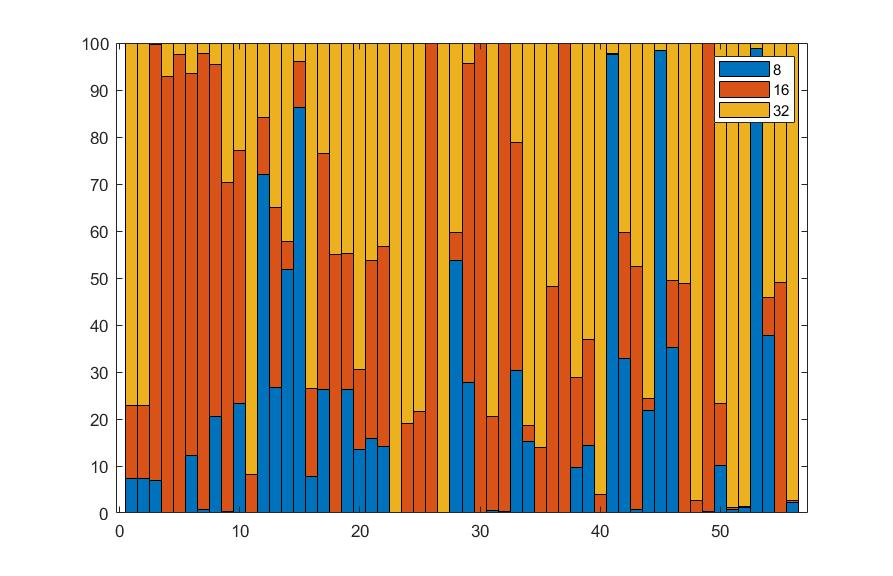
\includegraphics[width=.7\textwidth]{imagenes/chap4/delta_bar_row_porc_per_cat_32_rcm.jpg}
    \caption{Cada barra del gráfico simboliza una matriz que necesita 32 bits para ser representada luego de aplicar RCM, y cada componente es el porcentaje de deltas máximos por fila que pueden ser representadas con 8, 16 y 32 bits.}
    \label{fig:delta_bar_row_porc_per_cat_32_rcm}
\end{figure}

Tal y como se ha realizado en las secciones previas, a continuación se intenta ahondar en las matrices representables con 32 bits, las que poseen posiblemente, (a nuestro criterio mayor) interés. Se presenta en la Figura~\ref{fig:delta_bar_row_porc_per_cat_32_rcm}, un gráfico donde se puede observar, para las 56 matrices ordenadas por cantidad de elementos no nulos, la proporción de filas que pueden ser representadas en las diferentes precisiones. Con un fenómeno muy similar a su contraparte sin ordenar, pero a mucho menor escala, se obtiene un resultado muy variado en la proporción de filas, mientras que las primeras, las de menor \textit{nnz}, presentan pocas filas que necesitan 32 bits. Luego, a medida que aumenta la cantidad de elementos no nulos, paulatinamente crece la proporción de filas que pueden ser representadas sólo con 32 bits.



\subsection{Resumen de la evaluación}

\begin{table}[h]
\centering
\begin{tabular}{|l||r|r|r|}
\hline
         Variante                              & 8   & 16  & 32  \\ \hline\hline
4.3.1. Índice de columna                & 116 & 931 & 360 \\ \hline
4.3.2. Diferencia a la diagonal        & 230 & 821 & 356 \\ \hline
4.3.3. Diferencia a la diagonal con RCM & 371 & 961 & 75  \\ \hline
4.3.4. Delta entre índices              & 347 & 841 & 219 \\ \hline
4.3.5. Delta entre índices con RCM      & 488 & 863 & 56  \\ \hline
\end{tabular}
\caption{Resumen de los resultados de clasificación de las diferentes estrategias evaluadas.}
\label{tab:resumen-resultados}
\end{table}

Para resumir y analizar los datos obtenidos, se presenta en la Tabla~\ref{tab:resumen-resultados} la clasificación del espacio de matrices utilizado, aplicando las diferentes técnicas anteriormente discutidas. 
De ésta se desprenden varios resultados. Probablemente la primera observación que surge analizando la columna de la cantidad de matrices que pertenecen a la categoría de 32 bits, es la reducción de dicha cantidad al aplicar cualquiera de las técnicas propuestas respecto a utilizar los índices originales, incluso sin aplicar reordenamientos como RCM. En el caso de diferencia a la diagonal la reducción no es tan notoria, sólo 4 matrices menos, mientras que utilizando el delta entre índices se obtiene resultados más favorables.

Como segunda observación, las técnicas de reordenamiento abordadas mejoran significativamente la clasificación de las matrices, fenómeno que puede ser observado en la reducción de la cantidad de matrices que se clasifican con 32 bits. 
Esto motiva a continuar profundizando acerca de las técnicas para compresión de matrices aplicando reordenamientos en el futuro.
Otra línea interesante es la exploración de herramientas para optimizar operaciones como la SpMV utilizando estas técnicas, explotando también las características de distintas arquitecturas de hardware.
% Hay que estudiar también, no sólo enfocados en el almacenamiento, herramientas (pensando principalmente en operaciones como SpMV) que sepan explotar dicha estructura (Y también en diferentes arquitecturas), evaluando como afecta, por ejemplo, en términos de accesos a memoria y si existe un cierto \textit{overhead} de descompresión.
A pesar de que RCM no es una heurística específicamente diseñada para reordenar matrices con el objetivo de reducir el espacio de almacenamiento, cabe destacar que los resultados obtenidos, aplicando esta técnica, resultan más que favorables. A esta misma conclusión llegaron múltiples autores en sus investigaciones, tal y como se presenta en el Capítulo~\ref{ch:estado-del-arte}.

